\chapter{周转圆组与周转球组}
\label{chap:dyn_epicycle}
\markboth{周转圆组与周转球组}{周转圆组与周转球组}

\begin{remark}[本章定位]\label{rem:dyn_chapter_positioning}
本章紧接「矢量分析」章，把该章建立的静态三组投影模型推广为动态模型，并补齐单组动态、四元数单球组与旋转球组三类对象。全章遵循统一的两步结构：
\[
\textbf{合成} \;\longrightarrow\; \textbf{投影} \;\longrightarrow\; \textbf{观察结果}.
\]
\textbf{约定}：本章全部模型都采用“先合成、后投影”的顺序。即，首先把时间组与空间组合成为一个合成对象（复情形取加法 $T+S$，四元数情形取加法 $q_T+q_S$），然后把这个合成对象投影到观察者组上。观察者本身可以随时间变化，也可以按自身周转圆独立旋转。

\textbf{七主题导引}：平移——观察者向量的动态调节与频率平移；缩放——观察者模长引入的权重与包络对振幅的慢变调制；旋转——三平面与三球组的独立旋转；平衡——合成与投影的线性性；对称——投影的对称性与交换性；闭合——同步旋转的不变量；周期——动态投影的瞬时频率、拍频与包络周期。
\end{remark}

\begin{figure}[htbp]
\centering
\begin{tikzpicture}[
  font=\small,
  box/.style={draw, rounded corners, fill=blue!8, minimum width=2.6cm, minimum height=0.8cm, align=center},
  sub/.style={draw, rounded corners, fill=green!10, minimum width=2.4cm, minimum height=0.7cm, align=center, font=\footnotesize},
  arr/.style={->, thick, >=stealth}
]
  \node[box] (pre) {前置四级数\\振幅/频率/相位/周期};
  \node[box, right=0.9cm of pre] (single) {单组动态周转圆\\$\mathcal E(t)$};
  \node[box, right=0.9cm of single] (triple) {三组动态周转圆\\$T,S,O$};
  \node[box, right=0.9cm of triple] (rotating) {旋转三平面\\按内部周转圆旋转};
  \node[sub, below=1.0cm of pre] (quat) {四元数单球组\\$q_T,q_S,q_O$};
  \node[sub, below=1.0cm of single] (rotquat) {旋转三球组\\$r_jq_jr_j^{-1}$};
  \node[sub, below=1.0cm of triple] (unified) {统一观察者投影\\$\Pi_O(X)=\operatorname{Re}[X\overline O]$};
  \node[sub, below=1.0cm of rotating] (observer) {观察者函子\\伴随 $\Pi_O\dashv\Pi_O^*$};
  \node[sub, below=1.0cm of quat] (info) {投影信息压缩\\DPI 与率失真};

  \node[box, fill=orange!12] (extra) at ($(pre)!0.5!(rotating) + (0,-5.0)$)
       {离散幺正动态投影 + 尺度相关采样 + 信息随距离损失};
  \draw[arr] (pre) -- (single);
  \draw[arr] (single) -- (triple);
  \draw[arr] (triple) -- (rotating);
  \draw[arr] (pre) -- (quat);
  \draw[arr] (single) -- (rotquat);
  \draw[arr] (triple) -- (unified);
  \draw[arr] (rotating) -- (observer);
  \draw[arr] (quat) -- (info);
  \draw[arr] (rotquat) -- (extra);
  \draw[arr] (unified) -- (extra);
  \draw[arr] (observer) -- (extra);
  \draw[arr] (info) -- (extra);
\end{tikzpicture}
\caption{本章结构总览：从四级数前置出发，依次建立单组动态周转圆、三组动态周转圆、旋转三平面、四元数单球组、旋转三球组、统一观察者投影框架、观察者函子、投影信息压缩，最终汇集到离散幺正动态投影、尺度相关采样与信息随距离损失。}
\label{fig:dyn_overview}
\end{figure}

\section{前置：四级数与周转圆的定义}
\label{sec:dyn_prerequisites}

本节回顾「级数与卷积」章建立的振幅级数、频率级数、相位级数与周期级数，并在此基础上定义本章的基本对象——周转圆与周转球。本节的内容是对前序章节的引用与重组，不引入新的数学断言。

\subsection{振幅级数}

\begin{definition}[振幅级数（回顾）]\label{def:dyn_amplitude_series}
设振幅序列 $\{A_k\}_{k\in\mathbb Z}$ 满足 $A_k\ge 0$ 且 $\sum_k A_k<\infty$。称形式级数
\[
\mathcal A_f(t)=\sum_{k\in\mathbb Z}A_k e^{ikt}
\]
为\textbf{振幅级数}（实形式为 $\sum_k A_k\cos(kt)$，要求 $A_{-k}=A_k$）。振幅级数只保留振幅信息，丢弃相位与频率格结构。

\textbf{前提}：绝对可和 $\sum_k A_k<\infty$ 保证一致收敛（「级数与卷积」章 \cref{lem:absolute-summability-convergence}）。
\end{definition}

\begin{proposition}[振幅级数的玻尔均值系数公式（回顾）]\label{prop:dyn_amplitude_coefficient}
设 $\mathcal A_f(t)=\sum_k A_k e^{ikt}$ 一致绝对收敛，则对每个 $n\in\mathbb Z$，
\[
A_n=M\{\mathcal A_f(t)e^{-int}\}=\lim_{T\to\infty}\frac{1}{2T}\int_{-T}^{T}\mathcal A_f(t)e^{-int}\,dt.
\]
即振幅 $A_n$ 可由玻尔均值唯一提取。
\end{proposition}

\begin{proof}
由绝对可和性，玻尔均值可与求和交换：
\[
M\{\mathcal A_f(t)e^{-int}\}=\sum_k A_k M\{e^{i(k-n)t}\}.
\]
由指数基的正交性（「级数与卷积」章 \cref{lem:amplitude_exponential_mean}），$M\{e^{i(k-n)t}\}=\delta_{kn}$，故仅 $k=n$ 项保留，得 $A_n$。
\end{proof}

\subsection{频率级数}

\begin{definition}[频率级数（回顾）]\label{def:dyn_frequency_series}
设 $f$ 以 $T$ 为基本周期，频率格为 $\omega_n=2\pi n/T$。称形式级数
\[
\mathcal F_f(s)=\sum_{n\in\mathbb Z}\omega_n s^n=\frac{2\pi}{T}\sum_{n\in\mathbb Z}n s^n
\]
为\textbf{频率级数}。频率级数只保留频率格，丢弃振幅与相位。
\end{definition}

\begin{proposition}[频率级数与周期缩放（回顾）]\label{prop:dyn_frequency_scaling}
若 $f_\lambda(t):=f(t/\lambda)$（$\lambda>0$），则频率级数缩放为 $\mathcal F_{f_\lambda}(s)=\frac{1}{\lambda}\mathcal F_f(s)$。
\end{proposition}

\begin{proof}
$f_\lambda$ 以 $\lambda T$ 为周期，故其频率为 $\omega_n^{(\lambda)}=2\pi n/(\lambda T)=\omega_n/\lambda$，代入 \cref{def:dyn_frequency_series} 即得。
\end{proof}

\subsection{相位级数}

\begin{definition}[相位级数（回顾）]\label{def:dyn_phase_series}
设相位序列 $\{\phi_k\}_{k\in\mathbb Z}$。称形式级数
\[
\mathcal P_f(t)=\sum_{k\in\mathbb Z}e^{i(kt+\phi_k)}
\]
为\textbf{相位级数}。相位级数只保留相位，丢弃振幅与频率格。
\end{definition}

\begin{proposition}[相位级数与时间平移（回顾）]\label{prop:dyn_phase_translation}
时间平移 $f_\tau(t):=f(t-\tau)$ 使相位级数各项旋转 $-k\tau$：
\[
\mathcal P_{f_\tau}(t)=\sum_k e^{i(kt+\phi_k-k\tau)}.
\]
\end{proposition}

\begin{proof}
代入 $t\mapsto t-\tau$：$e^{i(k(t-\tau)+\phi_k)}=e^{i(kt+\phi_k-k\tau)}$，求和即得。
\end{proof}

\subsection{周期级数}

\begin{definition}[周期级数（回顾）]\label{def:dyn_periodic_series}
设 $P$ 为周期类指标集，$T_p>0$，四元组 $(A_{p,n},\omega_{p,n},\phi_{p,n},T_p)$ 满足 $\omega_{p,n}=2\pi n/T_p$。称
\[
f(t)=\sum_{p\in P}\sum_{n\in\mathbb Z}A_{p,n}e^{i(\omega_{p,n}t+\phi_{p,n})}
\]
为\textbf{周期级数}。周期级数以周期 $T_p$ 为一级指标，在每个周期层内由振幅级数提供 $A_{p,n}$、相位级数提供 $e^{i\phi_{p,n}}$、频率级数提供 $\omega_{p,n}$。
\end{definition}

\begin{proposition}[周期级数是四级数的综合（回顾）]\label{prop:dyn_periodic_synthesis}
周期级数由振幅、相位、频率与周期四个分量按周期层 $p$ 综合而成。单周期层 $P=\{T\}$ 时退化为傅里叶级数；进一步取相位为零或振幅为一分别得到振幅级数或相位级数。
\end{proposition}

\begin{proof}
由定义 \ref{def:dyn_periodic_series}，固定 $p$ 时内层和 $\sum_n A_{p,n}e^{i(\omega_{p,n}t+\phi_{p,n})}$ 是标准傅里叶级数。取 $P=\{T\}$ 得单层；取 $\phi_{p,n}\equiv0$ 得振幅级数；取 $A_{p,n}\equiv1$ 得相位级数。逐项核对即得。
\end{proof}

\subsection{周转圆：复平面内的周期单元}

\begin{definition}[周转圆]\label{def:dyn_epicycle}
设 $A>0$、$\omega\in\mathbb R$、$\phi\in[0,2\pi)$。称映射
\[
\gamma_{A,\omega,\phi}:\mathbb R\to\mathbb C,\qquad
\gamma_{A,\omega,\phi}(t)=A e^{i(\omega t+\phi)}
\]
为一个\textbf{周转圆}（epicycle）。三个参数分别称为\textbf{半径}（振幅）、\textbf{角速度}（频率）与\textbf{初相}。

\textbf{前提}：$A>0$。若 $A=0$，该周转圆退化为零映射。
\end{definition}

\begin{figure}[htbp]
\centering
\begin{tikzpicture}[scale=2.0,>=stealth]
  \draw[->] (-2.0,0) -- (2.0,0) node[right]{$\Re$};
  \draw[->] (0,-2.0) -- (0,2.0) node[above]{$\Im$};

  \draw[thick,blue] (0,0) circle (1.4);
  \draw[->,thick,blue] (0,0) -- (1.4,0) node[midway,below,font=\footnotesize]{$A$};
  \filldraw[blue] (1.4,0) circle (2pt);

  \draw[->,thick,red] (0.6,0) arc (0:60:0.6);
  \node[red,font=\footnotesize,xshift=0.5cm] at (0.7,0.35) {$\omega t+\phi$};
  \draw[->,thick,blue] (1.4,0) arc (0:120:1.4);
  \node[blue,font=\footnotesize] at (1.0,1.5) {$\gamma_{A,\omega,\phi}(t)$};
  \node[font=\footnotesize] at (0,-2.4) {复平面上的周转圆};
\end{tikzpicture}
\caption{周转圆：复平面上半径 $A$、角速度 $\omega$、初相 $\phi$ 的匀速圆周运动。}
\label{fig:dyn_epicycle}
\end{figure}

\begin{definition}[周转圆组]\label{def:dyn_epicycle_group_def}
设 $K\in\mathbb N^+$，$\{A_k\}_{k=1}^{K}\subset\mathbb R^+$，$\{\omega_k\}_{k=1}^{K}\subset\mathbb R$，$\{\phi_k\}_{k=1}^{K}\subset[0,2\pi)$。称有限和
\[
\mathcal E(t)=\sum_{k=1}^{K}A_k e^{i(\omega_k t+\phi_k)}
\]
为一个\textbf{周转圆组}。合成轨迹 $\mathcal E(t)$ 是复平面上的曲线。

\textbf{与四级数的关系}：\cref{def:dyn_epicycle_group_def} 是周期级数在单周期层、有限级数截断下的具体实现。其振幅由振幅级数给出（$\{A_k\}$），相位由相位级数给出（$\{\phi_k\}$），频率由频率级数给出（$\{\omega_k\}$），公共周期 $T=2\pi/\lvert\omega_0\rvert$（$\omega_0=\gcd\{\omega_k\ne0\}$ 为基频）由周期分量给出。
\end{definition}

\begin{figure}[htbp]
\centering
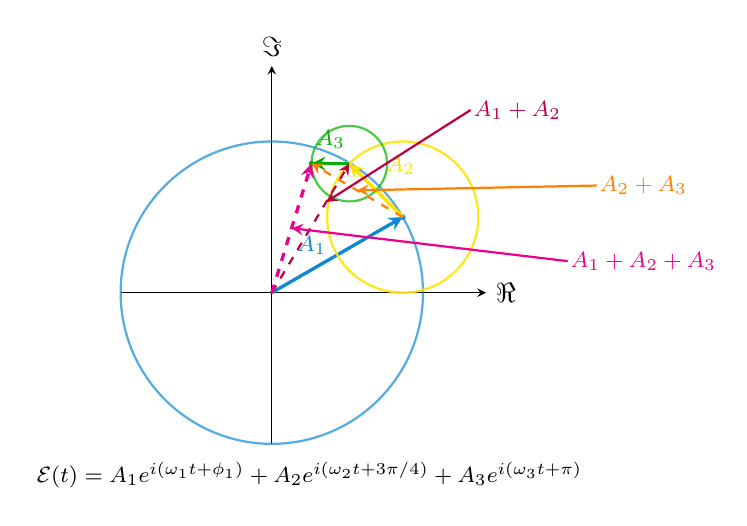
\begin{tikzpicture}[scale=1.6,>=stealth,
  lbl/.style={font=\footnotesize, inner sep=1pt}]

  \draw[->] (-1.2,0) -- (1.7,0) node[right]{$\Re$};
  \draw[->] (0,-1.2) -- (0,1.8) node[above]{$\Im$};

  \draw[thick,cyan!70!blue,opacity=0.7] (0,0) circle (1.2);
  \draw[->,very thick,cyan!70!blue] (0,0) -- (1.0392,0.6)
       node[lbl, pos=0.45, above left]{$A_1$};
  \filldraw[cyan!70!blue] (1.0392,0.6) circle (0.5pt);

  \draw[thick,yellow!85!orange,opacity=0.9] (1.0392,0.6) circle (0.6);
  \draw[->,very thick,yellow!85!orange] (1.0392,0.6) -- (0.6149,1.0243)
       node[lbl, pos=0.55, above right, xshift=3pt, yshift=3pt]{$A_2$};
  \filldraw[yellow!85!orange] (0.6149,1.0243) circle (0.5pt);

  \draw[thick,green!70!black,opacity=0.7] (0.6149,1.0243) circle (0.3);
  \draw[->,very thick,green!70!black] (0.6149,1.0243) -- (0.3149,1.0243)
       node[lbl, pos=0.5, above, yshift=4pt]{$A_3$};
  \filldraw[green!70!black] (0.3149,1.0243) circle (0.5pt);

  \draw[->,thick,purple,dashed]  (0,0)         -- (0.6149,1.0243);
  \draw[->,thick,orange,dashed]  (1.0392,0.6)  -- (0.3149,1.0243);
  \draw[->,very thick,magenta,dashed] (0,0)    -- (0.3149,1.0243);

  \node[lbl, purple]  (lbl12)  at (1.95, 1.45) {$A_1+A_2$};
  \draw[->, thick, purple]  (lbl12.west)  -- (0.43, 0.72);

  \node[lbl, orange]  (lbl23)  at ([xshift=1cm]1.95, 0.85) {$A_2+A_3$};
  \draw[->, thick, orange]  (lbl23.west)  -- (0.677, 0.812);

  \node[lbl, magenta] (lbl123) at ([xshift=1cm]1.95, 0.25) {$A_1+A_2+A_3$};
  \draw[->, thick, magenta] (lbl123.west) -- (0.157, 0.512);

  \node[font=\footnotesize] at (0.3,-1.45)
    {$\mathcal E(t)=A_1e^{i(\omega_1t+\phi_1)}+A_2e^{i(\omega_2t+3\pi/4)}+A_3e^{i(\omega_3t+\pi)}$};
\end{tikzpicture}
\caption{周转圆组：臂 $A_1$（天蓝，长度 $r_1$）位于圆 $A_1$ 内，臂 $A_2$（黄，长度 $r_2$，相位 $135^\circ$）位于圆 $A_2$ 内，臂 $A_3$（绿，长度 $r_3$，相位 $\pi$）位于圆 $A_3$ 内；各臂终点即下一级圆的圆心。三条合成向量 $A_1+A_2$（紫虚线）、$A_2+A_3$（橙虚线）、$A_1+A_2+A_3$（洋红虚线）为各级合成轨迹的瞬时值；它们的文字标识置于图形右侧外部，由同色箭头指向对应虚线。}
\label{fig:dyn_epicycle_group}
\end{figure}

\begin{proposition}[周转圆组的周期条件]\label{prop:dyn_epicycle_period_condition}
设 $\mathcal E(t)=\sum_{k=1}^{K}A_k e^{i(\omega_k t+\phi_k)}$ 且 $A_k>0$ 对所有 $k$ 成立。则 $\mathcal E$ 是周期函数当且仅当所有 $\omega_k$ 生成离散子群。此时记
\[
\omega_0:=\min\{\omega>0:\omega\in\textstyle\sum_k\mathbb{Z}\omega_k\}=\gcd\{\omega_k\ne0\},
\]
（即 $\omega_k/\omega_0\in\mathbb Z$ 对所有 $k$ 成立），则最小正周期为 $2\pi/\lvert\omega_0\rvert$（当 $\omega_0\notin\Omega$ 时为其整数分之一）；所有 $\omega_k=0$ 时不存在最小正周期。
\end{proposition}

\begin{proof}
\textbf{充分性}。若 $\omega_k=n_k\omega_0$（$n_k\in\mathbb Z$），则
\[
\mathcal E(t+T)=\sum_k A_k e^{i(n_k\omega_0(t+2\pi/\omega_0)+\phi_k)}
=\sum_k A_k e^{i(n_k\omega_0 t+\phi_k+2\pi n_k)}
=\sum_k A_k e^{i(n_k\omega_0 t+\phi_k)}=\mathcal E(t).
\]

\textbf{必要性}。若 $\mathcal E$ 以 $T>0$ 为周期，则对每个 $k$，$e^{i\omega_k T}=1$，即 $\omega_k T\in 2\pi\mathbb Z$。取 $\omega_0=2\pi/T$，则 $\omega_k/\omega_0=\omega_k T/(2\pi)\in\mathbb Z$。故所有频率是 $\omega_0$ 的整数倍。
\end{proof}

\begin{remark}[与静态模型的衔接]\label{rem:dyn_epicycle_static_link}
\cref{def:dyn_epicycle_group_def} 与「矢量分析」章所建立的嵌套周转圆组在数学对象上一致——它们都是复平面上的有限个复指数之和。本章的新内容在于：把这些周转圆的参数视为可随时间变化的函数，并研究由此产生的动态投影。
\end{remark}

\subsection{周转球：四元数空间内的周期单元}

\begin{definition}[周转球]\label{def:dyn_epicycle_ball}
设 $a>0$，$\mathbf u$ 为单位纯虚四元数（$\mathbf u^2=-1$），$\theta\in\mathbb R$。称映射
\[
\beta_{a,\mathbf u,\theta}:\mathbb R\to\mathbb H,\qquad
\beta_{a,\mathbf u,\theta}(t)=a\,e^{\mathbf u\theta t}
\]
为一个\textbf{周转球}（epicycle ball）。其中 $e^{\mathbf u\theta t}=\cos(\theta t)+\mathbf u\sin(\theta t)$ 为四元数指数。

三个参数分别称为\textbf{半径}（$a$）、\textbf{旋转轴}（$\mathbf u$）与\textbf{角速度}（$\theta$）。
\end{definition}

\begin{figure}[htbp]
\centering
\begin{tikzpicture}[scale=1.0,>=stealth]
  \draw[->] (-2.2,0) -- (2.2,0) node[right]{$\mathbf i$};
  \draw[->] (0,-2.2) -- (0,2.2) node[above]{$\mathbf j$};

  \draw[thick,blue,dashed] (0,0) circle (1.5);
  \draw[thick,blue] (0,0) ellipse (1.5 and 0.55);
  \draw[thick,blue] (0,0) ellipse (0.55 and 1.5);

  \draw[->,thick,red] (0,0) -- (1.2,0.9) node[above right,font=\footnotesize]{$a e^{\mathbf u\theta t}$};
  \filldraw[red] (1.2,0.9) circle (2pt);

  \draw[->,thick,green!60!black] (0,0) -- (0.5,-1.2) node[below,font=\footnotesize,xshift=0.5cm,yshift=-0.5cm]{$\mathbf u$};

  \node[blue,font=\footnotesize,xshift=-1cm,yshift=1cm] at (1.8,1.3) {$S^3_a$};
  \node[font=\footnotesize] at (0,-2.6) {周转球：四元数空间中的球面运动};
\end{tikzpicture}
\caption{周转球：四元数空间中半径 $a$ 的轨道位于三维球面 $S^3_a$ 上。}
\label{fig:dyn_epicycle_ball}
\end{figure}

\begin{definition}[周转球组]\label{def:dyn_epicycle_ball_group_def}
设 $K\in\mathbb N^+$，$a_k>0$，$\mathbf u_k$ 为单位纯虚四元数，$\theta_k\in\mathbb R$。称有限和
\[
q(t)=\sum_{k=1}^{K}a_k e^{\mathbf u_k\theta_k t}
\]
为一个\textbf{周转球组}。
\end{definition}

\begin{figure}[htbp]
\centering
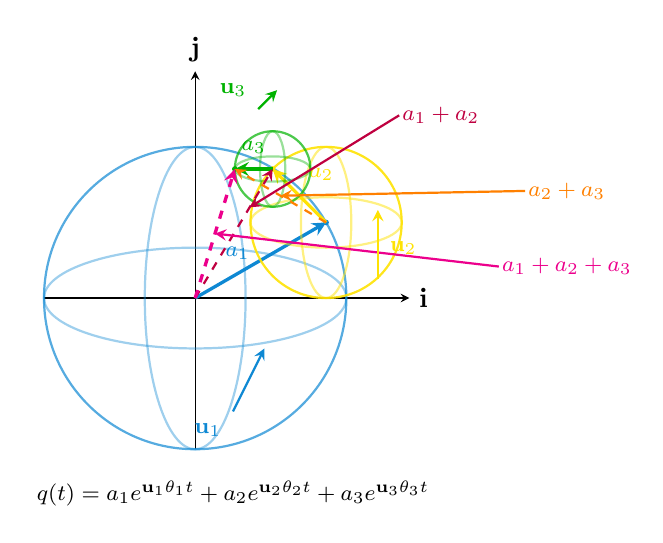
\begin{tikzpicture}[scale=1.6,>=stealth,
  lbl/.style={font=\footnotesize, inner sep=1pt}]

  \draw[->] (-1.2,0) -- (1.7,0) node[right]{$\mathbf i$};
  \draw[->] (0,-1.2) -- (0,1.8) node[above]{$\mathbf j$};

  \draw[thick,cyan!70!blue,opacity=0.7] (0,0) circle (1.2);
  \draw[thick,cyan!70!blue,opacity=0.4] (0,0) ellipse (1.2 and 0.4);
  \draw[thick,cyan!70!blue,opacity=0.4] (0,0) ellipse (0.4 and 1.2);
  \draw[->,very thick,cyan!70!blue] (0,0) -- (1.0392,0.6)
       node[lbl, pos=0.45, above left]{$a_1$};
  \filldraw[cyan!70!blue] (1.0392,0.6) circle (0.5pt);

  \draw[thick,yellow!85!orange,opacity=0.9] (1.0392,0.6) circle (0.6);
  \draw[thick,yellow!85!orange,opacity=0.5] (1.0392,0.6) ellipse (0.6 and 0.2);
  \draw[thick,yellow!85!orange,opacity=0.5] (1.0392,0.6) ellipse (0.2 and 0.6);
  \draw[->,very thick,yellow!85!orange] (1.0392,0.6) -- (0.6149,1.0243)
       node[lbl, pos=0.55, above right, xshift=3pt, yshift=3pt]{$a_2$};
  \filldraw[yellow!85!orange] (0.6149,1.0243) circle (0.5pt);

  \draw[thick,green!70!black,opacity=0.7] (0.6149,1.0243) circle (0.3);
  \draw[thick,green!70!black,opacity=0.4] (0.6149,1.0243) ellipse (0.3 and 0.1);
  \draw[thick,green!70!black,opacity=0.4] (0.6149,1.0243) ellipse (0.1 and 0.3);
  \draw[->,very thick,green!70!black] (0.6149,1.0243) -- (0.3149,1.0243)
       node[lbl, pos=0.5, above, yshift=4pt]{$a_3$};
  \filldraw[green!70!black] (0.3149,1.0243) circle (0.5pt);

  \draw[->,thick,purple,dashed]  (0,0)         -- (0.6149,1.0243);
  \draw[->,thick,orange,dashed]  (1.0392,0.6)  -- (0.3149,1.0243);
  \draw[->,very thick,magenta,dashed] (0,0)    -- (0.3149,1.0243);

  \node[lbl, purple]  (lbl12)  at (1.95, 1.45) {$a_1+a_2$};
  \draw[->, thick, purple]  (lbl12.west)  -- (0.43, 0.72);

  \node[lbl, orange]  (lbl23)  at ([xshift=1cm]1.95, 0.85) {$a_2+a_3$};
  \draw[->, thick, orange]  (lbl23.west)  -- (0.677, 0.812);

  \node[lbl, magenta] (lbl123) at ([xshift=1cm]1.95, 0.25) {$a_1+a_2+a_3$};
  \draw[->, thick, magenta] (lbl123.west) -- (0.157, 0.512);

  \draw[->, thick, cyan!70!blue] (0.3,-0.9) -- (0.55,-0.4);
  \node[cyan!70!blue, font=\footnotesize] at (0.1,-1.05) {$\mathbf u_1$};

  \draw[->, thick, yellow!85!orange] (1.45,0.15) -- (1.45,0.7);
  \node[yellow!85!orange, font=\footnotesize] at (1.65,0.4) {$\mathbf u_2$};

  \draw[->, thick, green!70!black] (0.5,1.5) -- (0.65,1.65);
  \node[green!70!black, font=\footnotesize] at (0.3,1.65) {$\mathbf u_3$};

  \node[font=\footnotesize] at (0.3,-1.55)
    {$q(t)=a_1e^{\mathbf u_1\theta_1t}+a_2e^{\mathbf u_2\theta_2t}+a_3e^{\mathbf u_3\theta_3t}$};
\end{tikzpicture}
\caption{周转球组：每个球的圆心落在上一级臂的终点，臂长等于对应球的半径；每个球用外圆加一横一竖两个椭圆表示 $S^3$ 球面。旋转轴 $\mathbf u_1,\mathbf u_2,\mathbf u_3$ 分别用同色箭头示意，体现四元数空间的非交换旋转。三条合成向量 $a_1+a_2$（紫虚线）、$a_2+a_3$（橙虚线）、$a_1+a_2+a_3$（洋红虚线）为各级合成路径的瞬时值。}
\label{fig:dyn_epicycle_ball_group}
\end{figure}

\begin{proposition}[周转球的范数]\label{prop:dyn_epicycle_ball_norm}
设 $\beta_{a,\mathbf u,\theta}(t)=a e^{\mathbf u\theta t}$。则对任意 $t$，
\[
|\beta_{a,\mathbf u,\theta}(t)|=a.
\]
即周转球在四元数空间中的轨道位于半径 $a$ 的三维球面 $S^3_a=\{q\in\mathbb H:|q|=a\}$ 上。
\end{proposition}

\begin{proof}
由 $e^{\mathbf u\theta t}=\cos(\theta t)+\mathbf u\sin(\theta t)$，计算范数：
\[
|e^{\mathbf u\theta t}|^2=\cos^2(\theta t)+|\mathbf u|^2\sin^2(\theta t)=\cos^2(\theta t)+\sin^2(\theta t)=1,
\]
其中用了 $|\mathbf u|=1$（单位纯虚四元数）与 $\mathbf u$ 与标量正交。故 $|\beta_{a,\mathbf u,\theta}(t)|=a|e^{\mathbf u\theta t}|=a$。
\end{proof}

\begin{remark}[周转球与四元数乘法的非交换性]\label{rem:dyn_epicycle_ball_noncommutative}
若两个周转球的旋转轴不同（$\mathbf u_1\neq\mathbf u_2$），则 $e^{\mathbf u_1\theta_1 t}e^{\mathbf u_2\theta_2 t}\neq e^{\mathbf u_2\theta_2 t}e^{\mathbf u_1\theta_1 t}$。这是四元数乘法的非交换性在周转球组上的直接体现，与复情形（$U(1)$ 交换）形成对比。
\end{remark}

\section{动态周转圆组}
\label{sec:dyn_single}

\subsection{基本定义}

\begin{definition}[动态周转圆组]\label{def:dyn_epicycle_group}
设 $K\in\mathbb N^+$。设振幅 $A_k:\mathbb R\to\mathbb R^+$、角频率 $\omega_k:\mathbb R\to\mathbb R$、相位 $\phi_k:\mathbb R\to\mathbb R$ 均为 $C^1$ 函数（$k=1,\dots,K$）。称
\[
\mathcal E(t)=\sum_{k=1}^{K}A_k(t)\,e^{i(\omega_k(t)t+\phi_k(t))}
\]
为一个\textbf{动态周转圆组}。若所有参数为常数，则退化为 \cref{def:dyn_epicycle_group_def}。

\textbf{前提}：$K$ 在紧区间上有限。允许 $K$ 在有限个时刻跳变的情形，见注 \ref{rem:dyn_K_jump}。

\textbf{瞬时相位与瞬时频率}：第 $k$ 项的总相位为 $\Phi_k(t)=\omega_k(t)t+\phi_k(t)$，其瞬时频率为
\[
\dot\Phi_k(t)=\omega_k(t)+t\dot\omega_k(t)+\dot\phi_k(t).
\]
注意：当 $\omega_k$ 非常值时，瞬时频率不等于 $\omega_k(t)$。本章凡涉及频率平移的结论，均指\textbf{瞬时频率}的平移。
\end{definition}

\begin{definition}[时间分量与空间分量]\label{def:dyn_time_space_components}
设 $\mathcal E(t)$ 为 \cref{def:dyn_epicycle_group} 的动态周转圆组。定义其\textbf{时间分量} $T(t)$ 与\textbf{空间分量} $S(t)$ 为
\[
T(t)=\operatorname{Re}\mathcal E(t)=\sum_{k=1}^{K}A_k(t)\cos(\omega_k(t)t+\phi_k(t)),
\]
\[
S(t)=\operatorname{Im}\mathcal E(t)=\sum_{k=1}^{K}A_k(t)\sin(\omega_k(t)t+\phi_k(t)).
\]
在复平面中，时间分量沿实轴、空间分量沿虚轴，二者自动正交。
\end{definition}

\begin{definition}[动态观察者向量]\label{def:dyn_observer}
设 $\theta:\mathbb R\to\mathbb R$ 为 $C^1$ 函数。称单位复数
\[
u(t)=e^{i\theta(t)}
\]
为\textbf{动态观察者向量}。$\theta(t)$ 称为观察者的\textbf{瞬时方向角}。
\end{definition}

\begin{definition}[动态投影观察结果]\label{def:dyn_projection}
设 $\mathcal E$ 为动态周转圆组，$u$ 为动态观察者向量。定义\textbf{观察结果}为
\[
\boxed{\ \mathcal O(t)=\operatorname{Re}\!\big[\mathcal E(t)\,\overline{u(t)}\big]\ }.
\]
由 \cref{def:dyn_time_space_components}，
\[
\mathcal O(t)=T(t)\cos\theta(t)+S(t)\sin\theta(t)
=\big\langle (T(t),S(t)),\,(\cos\theta(t),\sin\theta(t))\big\rangle.
\]
即观察结果是时间-空间二维实向量在动态观察者方向上的投影。
\end{definition}

\begin{figure}[htbp]
\centering
\begin{tikzpicture}[scale=1.0,>=stealth]
  \draw[->, thick] (-2.5,0) -- (3.5,0) node[right]{$T$};
  \draw[->, thick] (0,-2.5) -- (0,2.5) node[above]{$S$};

  \draw[->,very thick,red] (0,0) -- (2.0,1.4)
      node[above right=2pt,font=\footnotesize]{$\mathcal E(t)$};

  \draw[->,thick,blue] (0,0) -- (2.4,0.7)
      node[above=3pt,font=\footnotesize]{$u(t)=e^{i\theta(t)}$};

  \draw[gray,dashed] (2.0,1.4) -- (2.22,0.65);

  \draw[->,thick,orange] (0,0) -- (2.22,0.65);
  \node[orange,font=\footnotesize] at (1.0,-0.35) {$\mathcal O(t)$};

  \draw[->,thick] (0.9,0) arc (0:16:0.9);
  \node[font=\footnotesize] at (1.15,0.22) {$\theta(t)$};
\end{tikzpicture}
\caption{动态投影的几何图像：观察结果 $\mathcal O(t)$ 是源向量 $\mathcal E(t)$ 在观察者方向 $u(t)$ 上的正交投影。}
\label{fig:dyn_projection_geometry}
\end{figure}

\subsection{基本性质}

\begin{proposition}[投影的线性性]\label{prop:dyn_projection_linearity}
固定 $\theta(t)$，映射 $\mathcal E\mapsto\mathcal O$ 关于 $\mathcal E$ 是实线性的：
\[
\mathcal O[\alpha\mathcal E_1+\beta\mathcal E_2]
=\alpha\mathcal O[\mathcal E_1]+\beta\mathcal O[\mathcal E_2],
\qquad \alpha,\beta\in\mathbb R.
\]
\end{proposition}

\begin{proof}
由复乘法的分配律，
\[
(\alpha\mathcal E_1+\beta\mathcal E_2)\overline u=\alpha\mathcal E_1\overline u+\beta\mathcal E_2\overline u.
\]
由实部函数的线性性，
\[
\operatorname{Re}[\alpha\mathcal E_1\overline u+\beta\mathcal E_2\overline u]
=\alpha\operatorname{Re}[\mathcal E_1\overline u]+\beta\operatorname{Re}[\mathcal E_2\overline u].
\]
\end{proof}

\begin{proposition}[投影的对称性]\label{prop:dyn_projection_symmetry}
对任意动态周转圆组 $\mathcal E$ 与动态观察者 $u$，
\[
\mathcal O(t)=\operatorname{Re}[\mathcal E(t)\overline{u(t)}]
=\operatorname{Re}[u(t)\overline{\mathcal E(t)}].
\]
\end{proposition}

\begin{proof}
对任意 $z\in\mathbb C$ 有 $\operatorname{Re}z=\operatorname{Re}\overline z$。取 $z=\mathcal E\overline u$：
\[
\operatorname{Re}[\mathcal E\overline u]=\operatorname{Re}\overline{[\mathcal E\overline u]}
=\operatorname{Re}[\overline{\mathcal E}\,u]=\operatorname{Re}[u\overline{\mathcal E}].
\]
\end{proof}

\begin{lemma}[静态退化的单频公式]\label{lem:dyn_single_freq}
取 $\mathcal E(t)=A e^{i\omega t}$（$A>0$，$\omega\in\mathbb R$），观察者 $u(t)=e^{i\omega_0 t}$。则
\[
\mathcal O(t)=A\cos\big((\omega-\omega_0)t\big).
\]
\end{lemma}

\begin{proof}
$\mathcal E(t)\overline{u(t)}=A e^{i\omega t}\cdot e^{-i\omega_0 t}=A e^{i(\omega-\omega_0)t}$，取实部即得。
\end{proof}

\begin{theorem}[动态投影的连续性]\label{thm:dyn_projection_continuity}
设 $A_k,\omega_k,\phi_k,\theta$ 均为 $C^1$ 函数。则观察结果 $\mathcal O(t)$ 为 $C^1$ 函数。进一步，若 $|\mathcal E(t)|\neq 0$，则 $\mathcal O(t)$ 的\textbf{瞬时频率}为
\[
\Omega_{\mathcal O}(t)=\frac{d}{dt}\arg\!\big(\mathcal E(t)\overline{u(t)}\big).
\]
在单频情形 $\mathcal E(t)=A e^{i\omega t}$、$u(t)=e^{i\omega_0 t}$ 下退化为 $\omega-\omega_0$。
\end{theorem}

\begin{proof}
\textbf{连续性}。由 \cref{def:dyn_time_space_components}，$T(t)$ 与 $S(t)$ 是 $C^1$ 函数 $A_k,\omega_k,\phi_k$ 的有限和与复合，故为 $C^1$。由 \cref{def:dyn_observer}，$\theta$ 为 $C^1$，从而 $\cos\theta$、$\sin\theta$ 均为 $C^1$。由 \cref{def:dyn_projection}，$\mathcal O=T\cos\theta+S\sin\theta$ 是 $C^1$ 函数的乘积之和，故为 $C^1$。

\textbf{瞬时频率}。记 $z(t)=\mathcal E(t)\overline{u(t)}$，$\Phi(t)=\arg z(t)$。因 $|z(t)|=|\mathcal E(t)|\neq0$，$\Phi$ 局部可取连续分支且 $C^1$。由 $z=|z|e^{i\Phi}$，$\dot z=(|z|'+i|z|\dot\Phi)e^{i\Phi}$，故 $\dot\Phi=\operatorname{Im}(\dot z/z)$。单频情形由 \cref{lem:dyn_single_freq}，$z(t)=A e^{i(\omega-\omega_0)t}$，$\Phi(t)=(\omega-\omega_0)t$（在连续分支上），故 $\Omega_{\mathcal O}=\omega-\omega_0$。
\end{proof}

\begin{corollary}[旋转参考系下的频率平移]\label{cor:dyn_doppler}
在单频情形 \cref{lem:dyn_single_freq} 中，观察者看到的频率是 $\omega_{\text{obs}}=\omega-\omega_0$。当 $\omega_0=\omega$ 时，观察结果为常数 $A$。
\end{corollary}

\begin{proof}
由 \cref{lem:dyn_single_freq}，$\mathcal O(t)=A\cos((\omega-\omega_0)t)$，其频率为 $|\omega-\omega_0|$。当 $\omega=\omega_0$ 时 $\mathcal O(t)\equiv A$。
\end{proof}

\begin{property}[动态投影的基本性质]\label{prop:dyn_projection_properties}
\begin{enumerate}[label=(\roman*)]
    \item \textbf{零点保持}：$\mathcal E(t)=0\Rightarrow\mathcal O(t)=0$。
    \item \textbf{幅值界}：$|\mathcal O(t)|\le|\mathcal E(t)|$。
    \item \textbf{观察者反号}：$\theta\mapsto\theta+\pi$ 使 $\mathcal O\mapsto-\mathcal O$。
    \item \textbf{观察者旋转}：$\theta\mapsto\theta+\theta_0$ 使 $\mathcal O(t)\mapsto\operatorname{Re}[\mathcal E(t)e^{-i\theta_0}]$。
\end{enumerate}
\end{property}

\begin{proof}
(i) $\mathcal E(t)=0$ 时 $\mathcal E(t)\overline{u(t)}=0$，实部为零。

(ii) $|\mathcal O(t)|=|\operatorname{Re}[\mathcal E(t)\overline{u(t)}]|\le|\mathcal E(t)\overline{u(t)}|=|\mathcal E(t)|\cdot|\overline{u(t)}|=|\mathcal E(t)|$。

(iii) $u(t)=e^{i(\theta(t)+\pi)}=-e^{i\theta(t)}$，故 $\mathcal E\overline u=-\mathcal E\overline{e^{i\theta}}$，取实部变号。

(iv) 代入 $u(t)=e^{i(\theta(t)+\theta_0)}$，得 $\mathcal E\overline u=\mathcal E e^{-i\theta}e^{-i\theta_0}$，取实部即得。
\end{proof}

\begin{example}[动态投影的单频实例]\label{ex:dyn_single_freq_example}
取 $\mathcal E(t)=2e^{i3t}$，观察者 $u(t)=e^{it}$。由 \cref{lem:dyn_single_freq}，$\mathcal O(t)=2\cos(2t)$。若改取 $u(t)=e^{i3t}$，则 $\mathcal O(t)\equiv 2$。
\end{example}

\begin{remark}[$K$ 跳变的情形]\label{rem:dyn_K_jump}
允许 $K$ 在有限个时刻跳变时，$\mathcal E$ 在跳变时刻一般不连续。此时 $\mathcal O$ 只能在 $C^1$ 分段意义下定义。若要求 $\mathcal O$ 全局连续，可附加跳变前后总和不变的条件，或在跳变处用插值平滑。此类条件属于工程约定，本章默认 $K$ 恒定。
\end{remark}

\section{包络与瞬时相位}
\label{sec:dyn_envelope}

前两节把周转圆组的\emph{合成}与\emph{投影}分开处理：$\mathcal E(t)$ 是合成对象，$\mathcal O(t)=\operatorname{Re}[\mathcal E(t)\overline{u(t)}]$ 是观察结果。本节补上二者之间的一个中间对象——\textbf{包络}。直观上，包络是快振荡外面那层慢变的振幅轮廓；数学上，它是合成对象在共同相位旋转下的不变量，也是所有观察者读数的上确界。拍频、调幅、波包与慢–快系统都以它为共同语言。

\subsection{定义与三种入口}

\begin{definition}[包络与瞬时相位]\label{def:dyn_envelope}
设 $\mathcal E:\mathbb R\to\mathbb C$ 为 \cref{def:dyn_epicycle_group} 的动态周转圆组，且 $\mathcal E(t)\neq0$。将其写成极坐标形式
\[
\mathcal E(t)=\varrho(t)\,e^{i\Theta(t)},\qquad \varrho(t)=|\mathcal E(t)|\ge0,
\]
其中 $\Theta(t)$ 为 $\arg\mathcal E(t)$ 的连续分支。称 $\varrho$ 为 $\mathcal E$ 的\textbf{包络}，$\Theta$ 为\textbf{瞬时相位}，$\dot\Theta$ 为\textbf{瞬时频率}。若存在载波频率 $\bar\omega>0$ 使
\[
\varepsilon:=\frac{\sup_{t}|\dot\varrho(t)|}{\bar\omega\inf_{t}\varrho(t)}\ll1,
\]
则称 $\mathcal E$ 为\textbf{慢包络信号}，$\varrho$ 为\textbf{慢包络}，$\varepsilon$ 为\textbf{调制小参数}。
\end{definition}

\begin{remark}[包络的三种入口]\label{rem:dyn_envelope_three_entries}
包络可以从三个角度进入：
\begin{enumerate}[label=(\roman*)]
    \item \textbf{模长入口}：$\varrho=|\mathcal E|$，即复振幅的模；
    \item \textbf{观察者入口}：$\varrho(t)=\sup_{\theta}\operatorname{Re}[\mathcal E(t)e^{-i\theta}]$，即所有观察者方向下读数的上确界（\cref{prop:dyn_envelope_sup}）；
    \item \textbf{解析信号入口}：对实信号 $s$，$\varrho=|s+i\mathcal H\{s\}|$，其中 $\mathcal H$ 为希尔伯特变换（\cref{prop:analytic_signal}）。
\end{enumerate}
当 $\mathcal E$ 只含正频率时，$\mathcal E$ 本身即 $\operatorname{Re}\mathcal E$ 的解析信号，三者一致；若 $\mathcal E$ 含负频率分量，则模长入口给出的 $\varrho$ 一般不再是通常意义上的包络，这正是下文要求 $\varepsilon\ll1$ 的原因。
\end{remark}

\subsection{包络是观察者读数的上确界}

\begin{proposition}[上确界与不变性]\label{prop:dyn_envelope_sup}
固定 $t$，记 $\mathcal O_\theta(t)=\operatorname{Re}[\mathcal E(t)e^{-i\theta}]$。则
\[
\varrho(t)=\sup_{\theta\in[0,2\pi)}\mathcal O_\theta(t),
\]
且上确界在 $\theta\equiv\Theta(t)\pmod{2\pi}$ 处取到。进一步，对任意常数 $\psi$，
\[
\bigl|e^{i\psi}\mathcal E(t)\bigr|=|\mathcal E(t)|,
\]
即包络是共同相位旋转 $U(1)$ 作用的不变量。
\end{proposition}

\begin{proof}
由 $\mathcal E=\varrho e^{i\Theta}$ 得 $\mathcal O_\theta=\varrho\cos(\Theta-\theta)$。固定 $t$，$\cos(\Theta-\theta)$ 在 $\theta=\Theta$ 处取最大值 $1$，故上确界为 $\varrho$。不变性由 $|e^{i\psi}\mathcal E|=|e^{i\psi}|\,|\mathcal E|=|\mathcal E|$ 得到。
\end{proof}

\begin{remark}[包络与投影的关系]\label{rem:dyn_envelope_vs_projection}
\cref{prop:dyn_projection_properties}(ii) 给出 $|\mathcal O(t)|\le|\mathcal E(t)|$。\cref{prop:dyn_envelope_sup} 把它加强为：$\varrho(t)$ 不但是 $\mathcal O$ 的上界，而且是\emph{可达}上界——总存在一个观察者方向恰好读到 $\varrho(t)$。因此包络是观察者无关的量，而观察结果依赖于观察者方向；二者的差别正是“快相位”被投影掉的部分。
\end{remark}

\subsection{单分量与双近频}

\begin{proposition}[单分量与拍]\label{prop:dyn_envelope_beat}
\begin{enumerate}[label=(\roman*)]
    \item 若 $\mathcal E(t)=Ae^{i(\omega t+\phi)}$（$A>0$），则 $\varrho\equiv A$，$\Theta=\omega t+\phi$。
    \item 若 $\mathcal E(t)=Ae^{i(\omega_1t+\phi_1)}+Ae^{i(\omega_2t+\phi_2)}$（$A>0$，$\omega_1\neq\omega_2$），记
    \[
    \Delta\omega=|\omega_1-\omega_2|,\qquad \bar\omega=\frac{\omega_1+\omega_2}{2},\qquad \Delta\phi=\phi_1-\phi_2,\qquad \bar\phi=\frac{\phi_1+\phi_2}{2},
    \]
    则
    \[
    \mathcal E(t)=2A\cos\Bigl(\frac{\Delta\omega\,t+\Delta\phi}{2}\Bigr)e^{i(\bar\omega t+\bar\phi)},
    \]
    \[
    \varrho(t)=2A\Bigl|\cos\Bigl(\frac{\Delta\omega\,t+\Delta\phi}{2}\Bigr)\Bigr|,
    \]
    其最小正周期为 $T_{\text{env}}=2\pi/\Delta\omega=T_{\text{beat}}$；带符号慢变因子 $\cos\bigl((\Delta\omega t+\Delta\phi)/2\bigr)$ 的周期为 $4\pi/\Delta\omega$，是 $T_{\text{env}}$ 的两倍。
\end{enumerate}
\end{proposition}

\begin{proof}
(i) 由 \cref{def:dyn_envelope} 直接得到。(ii) 由和差化积，
\[
Ae^{i(\omega_1t+\phi_1)}+Ae^{i(\omega_2t+\phi_2)}
=2A\cos\Bigl(\frac{(\omega_1-\omega_2)t+(\phi_1-\phi_2)}{2}\Bigr)e^{i\bigl(\frac{\omega_1+\omega_2}{2}t+\frac{\phi_1+\phi_2}{2}\bigr)}.
\]
取模即得 $\varrho$ 的表达式；$|\cos|$ 的周期为 $\pi$，故 $\varrho$ 的周期为 $2\pi/\Delta\omega$。
\end{proof}

\begin{figure}[htbp]
\centering
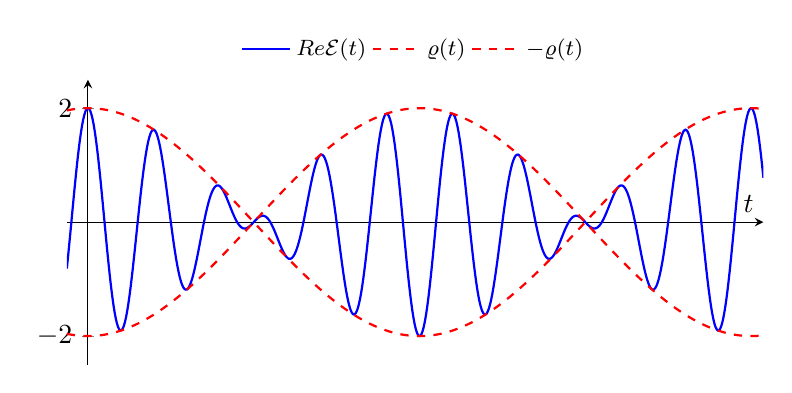
\begin{tikzpicture}
\begin{axis}[
  width=0.86\textwidth, height=5.2cm,
  axis lines=middle,
  xlabel={$t$},
  xmin=-0.4, xmax=12.8, ymin=-2.5, ymax=2.5,
  xtick=\empty, ytick={-2,0,2},
  samples=600, domain=-0.4:12.8,
  legend style={at={(0.5,1.03)},anchor=south,legend columns=3,draw=none,font=\footnotesize}
]
\addplot[blue,thick] {2*cos(deg(0.5*x))*cos(deg(5*x))};
\addplot[red,dashed,thick] {2*abs(cos(deg(0.5*x)))};
\addplot[red,dashed,thick] {-2*abs(cos(deg(0.5*x)))};
\legend{$\operatorname{Re}\mathcal E(t)$,$\varrho(t)$,$-\varrho(t)$}
\end{axis}
\end{tikzpicture}
\caption{双近频信号的包络：快载波被慢包络 $2A|\cos(\Delta\omega t/2)|$ 调制。此处 $A=1$，$\Delta\omega=1$，$\bar\omega=5$。}
\label{fig:dyn_envelope_beat}
\end{figure}

\begin{remark}[与音频、机械两章的口径]\label{rem:dyn_envelope_beat_convention}
「音频系统之周期结构」章与「机械系统之周期结构」章把“包络周期”记为 $4\pi/\Delta\omega$（\cref{lem:beat_periodic}、\cref{prop:beat_phenomenon}）。按 \cref{def:dyn_envelope}，那是\emph{带符号}慢变因子的周期；\emph{模}包络的周期是 $2\pi/\Delta\omega$，与拍周期 $T_{\text{beat}}=1/\Delta f$ 相等。引入本定义后，两处应统一为：拍周期等于模包络周期，带符号因子每两个拍周期才重复一次。
\end{remark}

\subsection{差频结构与包络的周期性}

\begin{theorem}[差频展开]\label{thm:dyn_envelope_difference}
设 $\mathcal E(t)=\sum_{k=1}^{K}A_ke^{i(\omega_kt+\phi_k)}$，其中 $K\ge2$，$A_k>0$ 为常数，$\omega_1,\dots,\omega_K$ 互不相同。则
\[
\varrho^2(t)=\sum_{k=1}^{K}A_k^2+2\sum_{1\le j<k\le K}A_jA_k\cos\bigl((\omega_j-\omega_k)t+(\phi_j-\phi_k)\bigr).
\]
记 $D$ 为上式右端系数非零的差频 $\omega_j-\omega_k$ 所生成的加法子群。则：
\begin{enumerate}[label=(\roman*)]
    \item $\varrho^2$ 的频谱只含差频；等价地，$\varrho^2$ 的频谱是载波频谱的自相关（离散维纳--辛钦关系）。
    \item 若 $D$ 离散且 $D=\omega_D\mathbb Z$（$\omega_D>0$），则 $\varrho$ 的最小正周期为 $T_{\text{env}}=2\pi/\omega_D$；若 $D$ 非离散，则 $\varrho$ 不是周期函数。
    \item 若全部 $\omega_k\in\omega_0\mathbb Z$，则 $T_{\text{env}}$ 整除载波周期 $T_c=2\pi/\omega_0$。
\end{enumerate}
\end{theorem}

\begin{proof}
由 $\varrho^2=\mathcal E\overline{\mathcal E}$ 展开：
\[
\mathcal E\overline{\mathcal E}=\sum_{j,k=1}^{K}A_jA_k e^{i((\omega_j-\omega_k)t+(\phi_j-\phi_k))}.
\]
把 $j=k$ 的 $K$ 项（每项 $A_k^2$）与 $j\ne k$ 的项分开，后者按 $(j,k)$ 与 $(k,j)$ 配对，利用 $e^{i\theta}+e^{-i\theta}=2\cos\theta$ 即得展开式。

(i) 由展开式直接读出。(ii) 展开式是有限三角多项式，其非零频率集合生成 $D$；三角多项式以 $T$ 为周期当且仅当每个非零频率 $\nu$ 满足 $\nu T\in2\pi\mathbb Z$（三角多项式频率的线性无关性）。故 $\varrho^2$ 的周期群为 $(2\pi/\omega_D)\mathbb Z$。又因 $\varrho=\sqrt{\varrho^2}\ge0$，$T$ 是 $\varrho^2$ 的周期当且仅当它是 $\varrho$ 的周期，故 $\varrho$ 与 $\varrho^2$ 的周期群相同，最小正周期为 $2\pi/\omega_D$。(iii) 若 $\omega_k\in\omega_0\mathbb Z$，则 $D\subseteq\omega_0\mathbb Z$，故 $\omega_D$ 是 $\omega_0$ 的正整数倍，$T_{\text{env}}=2\pi/\omega_D$ 整除 $2\pi/\omega_0$。
\end{proof}

\begin{corollary}[准周期载波可以有周期包络]\label{cor:dyn_envelope_quasiperiodic}
设 $\mathcal E(t)=Ae^{i\omega_1t}+Ae^{i\omega_2t}$，$A>0$，且 $\omega_1/\omega_2\notin\mathbb Q$。则 $\mathcal E$ 不是周期函数（它是玻尔准周期函数），但 $\varrho$ 以 $2\pi/|\omega_1-\omega_2|$ 为最小正周期。
\end{corollary}

\begin{proof}
两个不可公度频率的指数和没有非零周期：若 $T$ 是 $\mathcal E$ 的周期，则由三角多项式的频率独立性，$e^{i\omega_1T}=e^{i\omega_2T}=1$，故 $\omega_1T,\omega_2T\in2\pi\mathbb Z$，与 $\omega_1/\omega_2\notin\mathbb Q$ 矛盾。包络的周期性由 \cref{thm:dyn_envelope_difference}(ii) 给出，此时 $D=|\omega_1-\omega_2|\mathbb Z$。
\end{proof}

\begin{remark}[包络的周期性严格弱于载波的周期性]\label{rem:dyn_envelope_weaker}
\cref{cor:dyn_envelope_quasiperiodic} 说明：$\mathcal E$ 周期 $\Rightarrow$ $\varrho$ 周期（因 $\varrho=|\mathcal E|$），但反之不成立。群论上的原因很清楚：包络是共同相位旋转 $U(1)$ 的不变量（\cref{prop:dyn_envelope_sup}），它只看见\emph{相对相位} $\Theta_j-\Theta_k$，把共同的快相位商掉了。因此包络的周期是“相对相位的闭合周期”，它可以比载波周期更粗，也可以在载波根本没有周期时仍然存在。
\end{remark}

\subsection{周期差密度}
\label{subsec:dyn_period_difference_density}

本节把“两个周期函数的周期差”写成一个可积的密度。目标有两条：
\begin{enumerate}[label=(\roman*)]
    \item \textbf{逐点}：给定 \(f,g\) 与点 \(x\)，返回 \(x\) 处的周期差密度；
    \item \textbf{积分}：在区间 \([a,b]\) 上积分，返回该区间的周期差。
\end{enumerate}
这两条要求决定了逐点值不能是“周期”本身，而必须是无量纲的密度，并且依赖区间归一化。

\begin{remark}[为什么逐点值不能是周期]
\label{rem:dyn_period_density_no_go}
如果 \(D(x)\) 是周期（量纲为时间），那么 \(\int_a^b D(x)\,dx\) 的量纲是时间\(^2\)，不可能等于周期差（时间）。更严格地说，若固定 \(D(x)\) 且对任意区间 \([a,b]\) 都有
\[
\int_a^b D(x)\,dx=T_f-T_g,
\]
则对任意子区间积分都等于同一个常数；对 \(b\) 求导得 \(D(b)=0\) 对几乎所有 \(b\) 成立，矛盾。因此逐点值必须是无量纲密度，区间归一化不可避免；“区间上的周期差”应理解为区间平均周期之差，或“每过一个拍累积一个周期差”。
\end{remark}

\textbf{一般区间版。}

设 \(f,g\) 的全局最小正周期为 \(T_f,T_g\)，约定 \(T_f>T_g\)（否则交换 \(f,g\)）。解析相位为 \(\Theta_f,\Theta_g\)，局部频率为
\[
f_f(x)=\frac{\dot\Theta_f(x)}{2\pi},\qquad
f_g(x)=\frac{\dot\Theta_g(x)}{2\pi}.
\]
在区间 \([a,b]\) 上定义周期数
\[
N_f=\int_a^b f_f(x)\,dx,\qquad
N_g=\int_a^b f_g(x)\,dx,
\]
以及区间平均周期
\[
T_f^{[a,b]}=\frac{b-a}{N_f},\qquad
T_g^{[a,b]}=\frac{b-a}{N_g}.
\]

\begin{definition}[频率差密度与区间周期差密度]
\label{def:dyn_period_difference_density}
称
\[
\Delta_{f,g}(x)=f_g(x)-f_f(x)
\]
为 \(f,g\) 的\textbf{频率差密度}；称
\[
D_{f,g}(x;a,b)=\frac{b-a}{N_fN_g}\Delta_{f,g}(x)
\]
为 \(f,g\) 在区间 \([a,b]\) 上的\textbf{周期差密度}。
\end{definition}

\begin{proposition}[区间积分]
\label{prop:dyn_period_difference_integral}
对任意区间 \([a,b]\)，
\[
\int_a^b D_{f,g}(x;a,b)\,dx
=(b-a)\left(\frac1{N_f}-\frac1{N_g}\right)
=T_f^{[a,b]}-T_g^{[a,b]}.
\]
\end{proposition}

\begin{proof}
由 \(D_{f,g}\) 的定义，
\[
\int_a^b D_{f,g}(x;a,b)\,dx
=\frac{b-a}{N_fN_g}\int_a^b\Delta_{f,g}(x)\,dx
=\frac{b-a}{N_fN_g}(N_g-N_f),
\]
整理即得 \((b-a)(1/N_f-1/N_g)=T_f^{[a,b]}-T_g^{[a,b]}\)。
\end{proof}

\textbf{拍周期特例。}

取共同区间为一个拍周期
\[
T_{\rm env}=\frac{T_fT_g}{T_f-T_g},
\]
则 \(N_f=T_{\rm env}/T_f\)、\(N_g=T_{\rm env}/T_g\)，且 \(N_g-N_f=1\)。归一化因子化为
\[
\frac{T_{\rm env}}{N_fN_g}=T_f-T_g,
\]
密度变成
\[
D_{f,g}(x)=(T_f-T_g)\bigl(f_g(x)-f_f(x)\bigr),
\]
并且
\[
\int_0^{T_{\rm env}}D_{f,g}(x)\,dx
=(T_f-T_g)(N_g-N_f)=T_f-T_g.
\]
更一般地，区间含 \(m\) 个拍周期时，积分是 \(m(T_f-T_g)\)。这就是“每过一个拍，累积一个周期差”。

\textbf{包络的角色。}窄带/双单频时，包络 \(|z_f+z_g|\) 的周期正是 \(T_{\rm env}\)，它标记“相位差走完 \(2\pi\)”的区间（\cref{def:dyn_envelope}、\cref{prop:dyn_envelope_beat}）。包络给出积分域/时钟；局部频率（相位）给出逐点密度。只靠包络得不到 \(D_{f,g}(x)\)，只靠相位也得不到简洁的拍尺度，但可由 \(T_f,T_g\) 算出 \(T_{\rm env}\)。

\begin{example}[纯音检验]
\label{ex:dyn_period_difference_pure_tone}
对 \(f=\cos(2\pi x/T_f)\)、\(g=\cos(2\pi x/T_g)\)，有 \(f_f=1/T_f\)、\(f_g=1/T_g\)，所以
\[
D_{f,g}(x)=\frac{(T_f-T_g)^2}{T_fT_g}
\]
为常数；在 \(T_{\rm env}=T_fT_g/(T_f-T_g)\) 上积分：
\[
\frac{(T_f-T_g)^2}{T_fT_g}\cdot\frac{T_fT_g}{T_f-T_g}=T_f-T_g,
\]
与直接相减一致。
\end{example}

\begin{remark}[任意周期函数的校准]
\label{rem:dyn_period_density_calibration}
对谐波丰富或零点奇异的信号，解析相位的绕数可能不是 \(1\)。此时把 \(\dot\Theta/(2\pi)\) 换成\textbf{校准局部频率} \(f_f(x)\)，满足
\[
\int_0^{T_f} f_f(x)\,dx=1.
\]
可用 STFT 脊、自相关或“瞬时频率除以其在一个周期上的积分/绕数”得到。校准后，上面的积分恒等式不依赖解析相位的局部细节，只依赖总周期数。
\end{remark}

\begin{remark}[两种密度的分工]
\label{rem:dyn_two_densities}
\(\Delta_{f,g}\) 计数“多出的周期数”，是无量纲的频率差；\(D_{f,g}\) 把它乘以区间归一化因子 \((b-a)/(N_fN_g)\)，使其在 \([a,b]\) 上的积分成为区间周期差（在拍周期上该因子化为 \(T_f-T_g\)）。包络给出拍时钟 \(T_{\rm env}\)，相位差给出密度。历法章中的 \(D(t)=1/L_m-1/L_z\) 是 \(\Delta_{f,g}\) 的历法实例（用于计数闰余）；乘以相应的区间归一化因子即得 \(D_{f,g}\)，用于解释时间差。因此，周期差密度不是历法章特有的构造，而是解析信号的一般对象。
\end{remark}

\subsection{调制阶与公度}

\begin{definition}[调制阶]\label{def:dyn_modulation_order}
对 \cref{prop:dyn_envelope_beat}(ii) 的双分量信号，称
\[
N:=\frac{T_{\text{env}}}{T_c}=\frac{\bar\omega}{\Delta\omega}
\]
为\textbf{调制阶}，其中 $T_c=2\pi/\bar\omega$ 为载波周期。
\end{definition}

\begin{proposition}[调制阶与公度]\label{prop:dyn_modulation_order}
对 \cref{prop:dyn_envelope_beat}(ii) 的双分量信号：
\begin{enumerate}[label=(\roman*)]
    \item $\mathcal E$ 是周期函数当且仅当 $N\in\mathbb Q$；
    \item 若 $N=p/q$（$p,q$ 互素），则 $\mathcal E$ 的最小正周期为 $mT_{\text{env}}$，其中 $m$ 为正整数且 $m\mid 2q$。
\end{enumerate}
\end{proposition}

\begin{proof}
(i) $\mathcal E$ 是两个指数函数之和，其频率比为
\[
\frac{\omega_2}{\omega_1}=\frac{2N+1}{2N-1}.
\]
两个指数函数之和以 $T>0$ 为周期当且仅当 $\omega_1T,\omega_2T\in2\pi\mathbb Z$，这要求 $\omega_1/\omega_2\in\mathbb Q$；反之若 $\omega_1/\omega_2=r\in\mathbb Q$，取 $T=2\pi/\gcd(\omega_1,\omega_2)$ 即得周期。而 $(2N+1)/(2N-1)\in\mathbb Q$ 当且仅当 $N\in\mathbb Q$。

(ii) 取 $T_0=qT_{\text{env}}=2\pi q/\Delta\omega$。则 $\bar\omega T_0=2\pi qN=2\pi p$，$\Delta\omega T_0/2=\pi q$，故由 \cref{prop:dyn_envelope_beat}(ii) 的表达式，
\[
\mathcal E(t+T_0)=(-1)^q\mathcal E(t).
\]
于是 $2T_0=2qT_{\text{env}}$ 是 $\mathcal E$ 的周期。设 $\mathcal E$ 的最小正周期为 $P$。因 $P$ 也是 $\varrho$ 的周期，而 $\varrho$ 的最小正周期为 $T_{\text{env}}$，故 $P=mT_{\text{env}}$（$m\in\mathbb N^+$）。又 $P\mid 2qT_{\text{env}}$，故 $m\mid 2q$。
\end{proof}

\begin{remark}[与置闰、连分数的接口]\label{rem:dyn_envelope_intercalation}
\cref{prop:dyn_modulation_order} 把“双分量信号是否周期”化归为调制阶 $N$ 是否有理。$N$ 的无理程度可用其连分数收敛子 $p_j/q_j$ 度量：取 $N\approx p_j/q_j$ 时，信号在 $q_j$ 个包络周期内近似闭合，残余相位误差为 $2\pi q_j|N-p_j/q_j|$，由连分数理论不超过 $2\pi/q_{j+1}$。这与「离散采样逼近、同余角与置闰」章用连分数逼近周期比 $\varrho$（\cref{thm:continued_fraction_best_approx_parallel}）是同一类问题——前者逼近载波与包络之比，后者逼近采样窗与信号之比。
\end{remark}

\subsection{接口与开放问题}

\begin{remark}[与其他章的接口]\label{rem:dyn_envelope_interfaces}
包络在后续章节中以不同名义反复出现：
\begin{enumerate}[label=(\roman*)]
    \item \textbf{拍}（\cref{lem:beat_periodic}、\cref{prop:beat_phenomenon}）：双近频的模包络；
    \item \textbf{泄露包络}（\cref{thm:leakage_envelope_parallel}）：窗核旁瓣的衰减轮廓，是频域中的包络；
    \item \textbf{解析信号}（\cref{prop:analytic_signal}）：实信号的希尔伯特包络；
    \item \textbf{波包}（\cref{ex:dispersive_pulse}）：高斯脉冲的包络以群速度传播，色散作用于包络而非载波；
    \item \textbf{慢–快系统}（\cref{prop:pdo_enso_separation}）：慢变量对快振动振幅的调制，即包络动力学；
    \item \textbf{经济周期}：朱格拉周期对基钦周期振幅的调制（「经济系统之周期结构」章）。
\end{enumerate}
\end{remark}

\begin{remark}[开放问题]\label{rem:dyn_envelope_open}
\begin{enumerate}[label=(\alph*)]
    \item \textbf{多分量包络的唯一性}：当 $\mathcal E$ 含多个不可公度差频时，$\varrho$ 是准周期函数，如何定义其“包络的包络”？是否存在唯一的双尺度分解？
    \item \textbf{包络提取的误差界}：希尔伯特包络、峰值包络与 \cref{def:dyn_envelope} 的模长包络在有限采样下的误差如何定量刻画？
    \item \textbf{包络的范畴刻画}：包络作为 $U(1)$ 不变量的函子，能否纳入「周期范畴」章的框架？
\end{enumerate}
\end{remark}

\section{三组动态周转圆}
\label{sec:dyn_triple}

\subsection{基本定义}

\begin{definition}[三组动态周转圆]\label{def:dyn_triple_groups}
设三组彼此独立的动态周转圆组
\[
T(t)=\sum_{k=1}^{K_T}A_k(t)e^{i(\omega_k(t)t+\phi_k(t))},
\]
\[
S(t)=\sum_{l=1}^{K_S}B_l(t)e^{i(\nu_l(t)t+\psi_l(t))},
\]
\[
O(t)=\sum_{m=1}^{K_O}C_m(t)e^{i(\mu_m(t)t+\chi_m(t))},
\]
分别称为\textbf{时间组}、\textbf{空间组}、\textbf{观察者组}。三组参数均为 $C^1$ 函数。
\end{definition}

\begin{definition}[合成—投影观察结果]\label{def:dyn_triple_projection}
定义\textbf{合成轨迹}为 $T(t)+S(t)$，定义\textbf{观察结果}为合成轨迹在观察者组上的双线性配对之实部：
\[
\boxed{\ \mathcal O(t)=\operatorname{Re}\!\big[(T(t)+S(t))\,\overline{O(t)}\big]\ }.
\]
\end{definition}

\begin{remark}[与「矢量分析」章静态模型的关系]\label{rem:dyn_triple_static_relation}
\cref{def:dyn_triple_projection} 是「矢量分析」章三重静态投影模型的动态推广：当三组参数均为常数时，二者完全一致。
\end{remark}

\subsection{基本性质}

\begin{proposition}[合成—投影的可加性]\label{prop:dyn_triple_additivity}
观察结果关于时间组与空间组可加：
\[
\mathcal O(t)=\operatorname{Re}[T(t)\overline{O(t)}]+\operatorname{Re}[S(t)\overline{O(t)}].
\]
\end{proposition}

\begin{proof}
由复乘法分配律 $(T+S)\overline O=T\overline O+S\overline O$，再由实部线性性即得。
\end{proof}

\begin{proposition}[单位模观察者的退化]\label{prop:dyn_triple_unimodular}
若 $O(t)=e^{i\chi(t)}$，则 \cref{def:dyn_triple_projection} 退化为
\[
\mathcal O(t)=\operatorname{Re}\!\big[(T(t)+S(t))\,e^{-i\chi(t)}\big],
\]
与单组动态投影 \cref{def:dyn_projection} 的形式一致。
\end{proposition}

\begin{proof}
$|O(t)|=1$ 时 $\overline{O(t)}=O(t)^{-1}=e^{-i\chi(t)}$，代入即得。
\end{proof}

\begin{lemma}[双线性配对与模长权重]\label{lem:dyn_triple_weight}
一般情形下，
\[
\mathcal O(t)=\operatorname{Re}\!\big[(T(t)+S(t))\,\overline{\widehat O(t)}\big]\cdot|O(t)|,
\qquad \widehat O(t)=O(t)/|O(t)|.
\]
\end{lemma}

\begin{proof}
设 $\widehat O=O/|O|$，则 $O=|O|\widehat O$，$\overline O=|O|\overline{\widehat O}$。代入
\[
(T+S)\overline O=|O|\cdot(T+S)\overline{\widehat O}.
\]
取实部，$|O|\ge 0$ 为实数因子可提出即得。
\end{proof}

\begin{theorem}[三组动态投影的连续性]\label{thm:dyn_triple_continuity}
设 $T,S,O$ 的参数均为 $C^1$ 函数。则 $\mathcal O(t)$ 为 $C^1$ 函数。若 $O(t)\neq 0$ 对所有 $t$ 成立，则 $\mathcal O(t)$ 与 $|O(t)|$ 有相同的零点集。
\end{theorem}

\begin{proof}
\textbf{连续性}：$\mathcal O$ 是 $C^1$ 函数 $T,S,O$ 与其共轭的乘积再取实部，故为 $C^1$。

\textbf{零点集}：由 \cref{lem:dyn_triple_weight}，$\mathcal O=|O|\cdot\operatorname{Re}[(T+S)\overline{\widehat O}]$。若 $|O(t)|\neq 0$，则 $\mathcal O(t)=0$ 当且仅当 $\operatorname{Re}[(T+S)\overline{\widehat O}]=0$。
\end{proof}

\begin{corollary}[三组单频的拍频公式]\label{cor:dyn_triple_beat}
取 $T(t)=A e^{i\omega t}$、$S(t)=B e^{i\nu t}$、$O(t)=C e^{i\mu t}$（$A,B,C>0$）。则
\[
\mathcal O(t)=AC\cos((\omega-\mu)t)+BC\cos((\nu-\mu)t).
\]
当 $|\omega-\nu|$ 很小时产生拍频，拍周期为 $T_{\text{beat}}=2\pi/|\omega-\nu|$。
\end{corollary}

\begin{proof}
$T\overline O=AC e^{i(\omega-\mu)t}$，$S\overline O=BC e^{i(\nu-\mu)t}$，相加后取实部即得。
\end{proof}

\begin{property}[三组动态投影的基本性质]\label{prop:dyn_triple_properties}
\begin{enumerate}[label=(\roman*)]
    \item \textbf{线性性}：固定 $O$，$\mathcal O$ 关于 $T$ 与 $S$ 实线性。
    \item \textbf{观察者反号}：$O\mapsto-O$ 使 $\mathcal O\mapsto-\mathcal O$。
    \item \textbf{观察者共轭}：$O\mapsto\overline O$ 使 $\mathcal O\mapsto\operatorname{Re}[(T+S)O]$。
    \item \textbf{能量分解}：$|\mathcal O(t)|\le|T(t)+S(t)|\cdot|O(t)|$。
\end{enumerate}
\end{property}

\begin{proof}
(i) 由 \cref{prop:dyn_triple_additivity} 与复乘法关于第一因子的线性性。(ii) $\overline{-O}=-\overline O$。(iii) $\overline{\overline O}=O$。(iv) $|\mathcal O|\le|(T+S)\overline O|=|T+S|\cdot|O|$。
\end{proof}

\begin{example}[三组动态投影的拍频实例]\label{ex:dyn_triple_beat_example}
取 $T(t)=e^{i10t}$、$S(t)=e^{i12t}$、$O(t)=e^{i11t}$。由 \cref{cor:dyn_triple_beat}，
\[
\mathcal O(t)=\cos(-t)+\cos(t)=2\cos t.
\]
拍周期 $T_{\text{beat}}=2\pi$。
\end{example}

\begin{remark}[归一化与未归一化观察者]\label{rem:dyn_triple_normalisation}
若把观察者组归一化为 $\widehat O=O/|O|$，则 \cref{lem:dyn_triple_weight} 中的权重因子 $|O(t)|$ 消失，观察结果退化为真正的正交投影。是否归一化是建模选择。
\end{remark}

\section{旋转三平面}
\label{sec:dyn_rotating_planes}

\subsection{基本定义}

\begin{definition}[旋转三平面]\label{def:dyn_rotating_planes}
设三个彼此独立的复平面 $\mathbb C_T,\mathbb C_S,\mathbb C_O$。每个平面上有一组动态周转圆 $T_0(t),S_0(t),O_0(t)$（如 \cref{def:dyn_triple_groups}）。设 $\theta_T,\theta_S,\theta_O:\mathbb R\to\mathbb R$ 为 $C^1$ 函数。定义\textbf{旋转后的轨迹}为
\[
T(t)=T_0(t)e^{i\theta_T(t)},\quad
S(t)=S_0(t)e^{i\theta_S(t)},\quad
O(t)=O_0(t)e^{i\theta_O(t)}.
\]
三个平面的旋转角由对应平面内的周转圆组决定，故称“按内部周转圆的属性旋转”。
\end{definition}

\begin{figure}[htbp]
\centering
\begin{tikzpicture}[scale=0.9,>=stealth]
  % 三个复平面
  \begin{scope}[shift={(0,0)}]
    \draw[thick, fill=blue!5] (-1.8,-1.8) rectangle (1.8,1.8);
    \draw[->] (-1.8,0) -- (1.8,0);
    \draw[->] (0,-1.8) -- (0,1.8);
    \draw[thick,blue] (0,0) circle (1.3);
    \draw[->,thick,blue] (0,0) -- (1.3,0);
    \node[blue,font=\footnotesize] at (0,-2.2) {$\mathbb C_T$（时间）};
    \node[blue,font=\footnotesize] at (1.5,1.2) {$T_0$};
  \end{scope}
  \begin{scope}[shift={(5,0)}]
    \draw[thick, fill=green!5] (-1.8,-1.8) rectangle (1.8,1.8);
    \draw[->] (-1.8,0) -- (1.8,0);
    \draw[->] (0,-1.8) -- (0,1.8);
    \draw[thick,green!60!black] (0,0) circle (1.0);
    \draw[->,thick,green!60!black] (0,0) -- (0,1.0);
    \node[green!60!black,font=\footnotesize] at (0,-2.2) {$\mathbb C_S$（空间）};
    \node[green!60!black,font=\footnotesize] at (1.5,1.2) {$S_0$};
  \end{scope}
  \begin{scope}[shift={(10,0)}]
    \draw[thick, fill=red!5] (-1.8,-1.8) rectangle (1.8,1.8);
    \draw[->] (-1.8,0) -- (1.8,0);
    \draw[->] (0,-1.8) -- (0,1.8);
    \draw[thick,red] (0,0) circle (1.5);
    \draw[->,thick,red] (0,0) -- (-1.0,1.1);
    \node[red,font=\footnotesize] at (0,-2.2) {$\mathbb C_O$（观察者）};
    \node[red,font=\footnotesize] at (1.5,1.2) {$O_0$};
  \end{scope}
  % 旋转标注
  \draw[->,thick,orange] (0.3,0.3) arc (30:80:0.5);
  \node[orange,font=\footnotesize] at (0.7,0.5) {$\theta_T$};
  \draw[->,thick,orange] (5.3,0.3) arc (30:80:0.5);
  \node[orange,font=\footnotesize] at (5.7,0.5) {$\theta_S$};
  \draw[->,thick,orange] (10.3,0.3) arc (30:80:0.5);
  \node[orange,font=\footnotesize] at (10.7,0.5) {$\theta_O$};
\end{tikzpicture}
\caption{旋转三平面：三个独立的复平面各自按内部周转圆的属性旋转，旋转角为 $\theta_T,\theta_S,\theta_O$。}
\label{fig:dyn_rotating_planes}
\end{figure}

\begin{definition}[旋转三平面的观察结果]\label{def:dyn_rotating_planes_projection}
沿用 \cref{def:dyn_rotating_planes}。定义
\[
\boxed{\ \mathcal O(t)=\operatorname{Re}\!\big[(T(t)+S(t))\,\overline{O(t)}\big]\ }.
\]
展开：
\[
\mathcal O(t)=\operatorname{Re}\!\big[(T_0 e^{i\theta_T}+S_0 e^{i\theta_S})\,e^{-i\theta_O}\,\overline{O_0}\big].
\]
\end{definition}

\subsection{基本性质}

\begin{proposition}[旋转角的相位平移作用]\label{prop:dyn_rotation_phase_shift}
旋转三平面等价于在合成前对 $T_0,S_0,O_0$ 分别施加相位平移 $\theta_T,\theta_S,\theta_O$：
\[
\mathcal O(t)=\operatorname{Re}\!\big[(T_0 e^{i(\theta_T-\theta_O)}+S_0 e^{i(\theta_S-\theta_O)})\,\overline{O_0}\big].
\]
因此只有两个相对旋转角 $\theta_T-\theta_O$ 与 $\theta_S-\theta_O$ 起作用。
\end{proposition}

\begin{proof}
展开
\[
(T_0 e^{i\theta_T}+S_0 e^{i\theta_S})\overline{O_0 e^{i\theta_O}}
=(T_0 e^{i\theta_T}+S_0 e^{i\theta_S})\overline{O_0}e^{-i\theta_O}.
\]
将 $e^{-i\theta_O}$ 分配到每一项，得
\[
=T_0 e^{i(\theta_T-\theta_O)}\overline{O_0}+S_0 e^{i(\theta_S-\theta_O)}\overline{O_0}
=\big[T_0 e^{i(\theta_T-\theta_O)}+S_0 e^{i(\theta_S-\theta_O)}\big]\overline{O_0}.
\]
取实部即得。
\end{proof}

\begin{theorem}[同步旋转下的不变量]\label{thm:dyn_sync_invariance}
若 $\theta_T(t)=\theta_S(t)=\theta_O(t)=\theta(t)$，则观察结果与静态情形相同：
\[
\mathcal O(t)=\operatorname{Re}\!\big[(T_0(t)+S_0(t))\overline{O_0(t)}\big].
\]
\end{theorem}

\begin{proof}
代入 $\theta_T=\theta_S=\theta_O=\theta$，由 \cref{prop:dyn_rotation_phase_shift}，两个相对角均为零：
\[
T_0 e^{i0}+S_0 e^{i0}=T_0+S_0.
\]
故 $\mathcal O=\operatorname{Re}[(T_0+S_0)\overline{O_0}]$，与 $\theta$ 无关。
\end{proof}

\begin{corollary}[异步旋转下的频率平移]\label{cor:dyn_async_beat}
取三平面均为单频：$T_0=A e^{i\omega t}$、$S_0=B e^{i\nu t}$、$O_0=C e^{i\mu t}$，旋转角 $\theta_j(t)=\Omega_j t$。则
\[
\mathcal O(t)=AC\cos\big((\omega+\Omega_T-\mu-\Omega_O)t\big)+BC\cos\big((\nu+\Omega_S-\mu-\Omega_O)t\big).
\]
\end{corollary}

\begin{proof}
由 \cref{prop:dyn_rotation_phase_shift}，$T_0e^{i(\theta_T-\theta_O)}=A e^{i(\omega+\Omega_T-\Omega_O)t}$，$S_0e^{i(\theta_S-\theta_O)}=B e^{i(\nu+\Omega_S-\Omega_O)t}$。代入取实部即得。
\end{proof}

\begin{property}[旋转三平面的基本性质]\label{prop:dyn_rotating_planes_properties}
\begin{enumerate}[label=(\roman*)]
    \item \textbf{相对性}：观察结果只依赖相对旋转角 $\theta_T-\theta_O$ 与 $\theta_S-\theta_O$。
    \item \textbf{同步不变性}：三平面同步旋转时观察结果不变。
    \item \textbf{频率平移}：若 $\theta_j=\Omega_j t$，则平面 $j$ 内所有分量频率整体平移 $\Omega_j$。
\end{enumerate}
\end{property}

\begin{proof}
(i)(ii) 由 \cref{prop:dyn_rotation_phase_shift} 与 \cref{thm:dyn_sync_invariance}。(iii) 由 $e^{i(\omega_j t+\Omega_j t)}=e^{i(\omega_j+\Omega_j)t}$ 直接得出。
\end{proof}

\begin{example}[三平面异步旋转的拍频实例]\label{ex:dyn_rotating_planes_example}
取 $T_0=e^{i10t}$、$S_0=e^{i12t}$、$O_0=e^{i11t}$，$\theta_T=0.5t$、$\theta_S=0$、$\theta_O=0$。由 \cref{cor:dyn_async_beat}，
\[
\mathcal O(t)=\cos(-0.5t)+\cos(t).
\]
两项频率分别为 $0.5$ 与 $1$，产生慢拍。
\end{example}

\begin{remark}[旋转角的选择]\label{rem:dyn_rotation_angle_choice}
“按内部周转圆属性旋转”有多种实现：$\theta_j(t)=\omega_{j,1}(t)t$、$\theta_j(t)=\arg X_j(t)$、$\theta_j(t)=\sum_k\omega_{j,k}(t)t$ 等。本章不固定其中一种，所有结论对任意 $C^1$ 旋转角成立。
\end{remark}

\section{四元数周转球组}
\label{sec:dyn_quaternion_single}

\subsection{基本定义}

\begin{definition}[四元数周转球组]\label{def:dyn_quaternion_group}
设 $K_T,K_S,K_O\in\mathbb N^+$。设 $a_k,b_l,c_m:\mathbb R\to\mathbb R$ 为 $C^1$ 实值函数；$\mathbf u_k,\mathbf v_l,\mathbf w_m:\mathbb R\to S^2$ 为 $C^1$ 单位纯虚四元数取值函数；$\theta_k,\psi_l,\chi_m:\mathbb R\to\mathbb R$ 为 $C^1$ 函数。定义
\[
q_T(t)=\sum_{k=1}^{K_T}a_k(t)e^{\mathbf u_k(t)\theta_k(t)},\quad
q_S(t)=\sum_{l=1}^{K_S}b_l(t)e^{\mathbf v_l(t)\psi_l(t)},\quad
q_O(t)=\sum_{m=1}^{K_O}c_m(t)e^{\mathbf w_m(t)\chi_m(t)}.
\]
分别称为\textbf{时间球组}、\textbf{空间球组}、\textbf{观察者球组}。
\end{definition}

\begin{definition}[合成—投影观察结果]\label{def:dyn_quaternion_projection}
定义合成向量为 $q_T(t)+q_S(t)$，观察结果为
\[
\boxed{\ \mathcal Q(t)=\operatorname{Re}\!\big[(q_T(t)+q_S(t))\,\overline{q_O(t)}\big]\ }.
\]
其中 $\overline{q_O}$ 为四元数共轭，$\operatorname{Re}$ 取四元数的标量部分。
\end{definition}

\begin{remark}[与「矢量分析」章静态模型的关系]\label{rem:dyn_quaternion_static_relation}
\cref{def:dyn_quaternion_projection} 是「矢量分析」章静态投影模型在“先合成再投影”约定下的动态版本。
\end{remark}

\subsection{基本性质}

\begin{proposition}[标量投影与共轭投影的区别]\label{prop:dyn_quaternion_projection_types}
四元数内积标量部分 $\operatorname{Re}[q\overline{p}]$ 与共轭作用 $p^{-1}qp$ 是两类不同的“投影”：
\begin{enumerate}[label=(\roman*)]
    \item $\operatorname{Re}[q\overline{p}]$ 是 $\mathbb R^4$ 上的内积投影，输出实数。
    \item $p^{-1}qp$ 是 $SO(3)$ 的旋转，输出四元数。
\end{enumerate}
本章采用 (i)。
\end{proposition}

\begin{proof}
(i) 由四元数内积定义 $\operatorname{Re}[q\overline p]=\sum_{i=0}^3 q_i p_i\in\mathbb R$。

(ii) 取 $q=\mathbf i$、$p=\mathbf j$。则 $p^{-1}=\overline p/|p|^2=-\mathbf j$，
\[
p^{-1}qp=(-\mathbf j)\mathbf i\mathbf j.
\]
由 $\mathbf i\mathbf j=\mathbf k$、$\mathbf j\mathbf i=-\mathbf k$：
\[
(-\mathbf j)\mathbf i\mathbf j=(-\mathbf j)(\mathbf i\mathbf j)=(-\mathbf j)\mathbf k=-\mathbf j\mathbf k=-\mathbf i.
\]
故 $p^{-1}qp=-\mathbf i\neq\mathbf i=q$，共轭作用改变四元数。
\end{proof}

\begin{lemma}[四元数内积的对称性]\label{lem:dyn_quaternion_inner_symmetry}
对任意 $p,q\in\mathbb H$，$\operatorname{Re}[p\overline q]=\operatorname{Re}[q\overline p]$。
\end{lemma}

\begin{proof}
$p\overline q$ 的标量部分为 $p_0q_0+p_1q_1+p_2q_2+p_3q_3$（矢量部分与非交换项不影响标量部分）。这是一个对称实双线性形式，故 $\operatorname{Re}[p\overline q]=\operatorname{Re}[q\overline p]$。
\end{proof}

\begin{theorem}[非交换合成与观察顺序]\label{thm:dyn_quaternion_noncommutative}
考虑加法合成 $X_+=q_T+q_S$ 与乘法合成 $X_\times=q_Tq_S$。则一般 $\operatorname{Re}[X_+\overline{q_O}]\neq\operatorname{Re}[X_\times\overline{q_O}]$，且 $q_Tq_S\neq q_Sq_T$。
\end{theorem}

\begin{proof}
取 $q_T=\mathbf i$、$q_S=\mathbf j$、$q_O=\mathbf k$。

加法：$X_+=\mathbf i+\mathbf j$，
\[
X_+\overline{q_O}=(\mathbf i+\mathbf j)(-\mathbf k)=-\mathbf i\mathbf k-\mathbf j\mathbf k.
\]
由 $\mathbf i\mathbf k=-\mathbf j$、$\mathbf j\mathbf k=\mathbf i$，得 $X_+\overline{q_O}=\mathbf j-\mathbf i$，标量部分为 $0$。

乘法：$X_\times=\mathbf i\mathbf j=\mathbf k$，
\[
X_\times\overline{q_O}=\mathbf k\cdot(-\mathbf k)=-\mathbf k^2=1,
\]
标量部分为 $1$。故两者不同。

非交换性：$\mathbf i\mathbf j=\mathbf k$，$\mathbf j\mathbf i=-\mathbf k$，故 $\mathbf i\mathbf j\neq\mathbf j\mathbf i$。
\end{proof}

\begin{corollary}[加法约定的交换性]\label{cor:dyn_quaternion_additive_commutative}
在加法约定下，$\operatorname{Re}[(q_T+q_S)\overline{q_O}]=\operatorname{Re}[(q_S+q_T)\overline{q_O}]$。
\end{corollary}

\begin{proof}
四元数加法交换。
\end{proof}

\begin{property}[四元数动态投影的基本性质]\label{prop:dyn_quaternion_properties}
\begin{enumerate}[label=(\roman*)]
    \item \textbf{实线性性}：固定 $q_O$，$\mathcal Q$ 关于 $q_T$ 与 $q_S$ 实线性。
    \item \textbf{观察者反号}：$q_O\mapsto-q_O$ 使 $\mathcal Q\mapsto-\mathcal Q$。
    \item \textbf{范数界}：$|\mathcal Q(t)|\le|q_T(t)+q_S(t)|\cdot|q_O(t)|$。
    \item \textbf{标量退化}：若四元数退化为复数，\cref{def:dyn_quaternion_projection} 退化为 \cref{def:dyn_triple_projection}。
\end{enumerate}
\end{property}

\begin{proof}
(i) 由四元数加法线性性、共轭反自同构性 $(p+q)^* = p^*+q^*$ 与标量部分线性性。

(ii) $\overline{-q_O}=-\overline{q_O}$，取标量部分变号。

(iii) $|\mathcal Q|=|\operatorname{Re}[(q_T+q_S)\overline{q_O}]|\le|(q_T+q_S)\overline{q_O}|=|q_T+q_S|\cdot|q_O|$。

(iv) 复数 $z=x+iy$ 嵌入四元数为 $x+y\mathbf i$，此时 $z_1\overline{z_2}$ 的标量部分与复情形内积实部一致。
\end{proof}

\begin{example}[单球组动态投影实例]\label{ex:dyn_quaternion_example}
取 $q_T=e^{\mathbf i t}$、$q_S=e^{\mathbf j t}$、$q_O=1$。则
\[
\mathcal Q(t)=\operatorname{Re}[e^{\mathbf i t}+e^{\mathbf j t}]=\cos t+\cos t=2\cos t.
\]
\end{example}

\begin{remark}[与复情形的对应]\label{rem:dyn_quaternion_complex_correspondence}
若所有四元数限制在同一复平面内，则非交换性消失，\cref{def:dyn_quaternion_projection} 完全退化为 \cref{def:dyn_triple_projection}。
\end{remark}

\section{旋转三球组}
\label{sec:dyn_quaternion_triple}

\subsection{基本定义}

\begin{definition}[旋转三球组]\label{def:dyn_rotating_quaternion_groups}
设三个彼此独立的四元数球组 $q_{T,0}(t),q_{S,0}(t),q_{O,0}(t)$。设 $r_T,r_S,r_O:\mathbb R\to S^3$ 为 $C^1$ 单位四元数取值函数。定义
\[
q_T(t)=r_T(t)\,q_{T,0}(t)\,r_T(t)^{-1},\quad
q_S(t)=r_S(t)\,q_{S,0}(t)\,r_S(t)^{-1},\quad
q_O(t)=r_O(t)\,q_{O,0}(t)\,r_O(t)^{-1}.
\]
\end{definition}

\begin{figure}[htbp]
\centering
\begin{tikzpicture}[scale=0.9,>=stealth]

  \begin{scope}[shift={(0,0)}]
    \draw[thick, fill=blue!5] (-1.8,-1.8) rectangle (1.8,1.8);
    \draw[thick,blue,dashed] (0,0) circle (1.4);
    \draw[thick,blue] (0,0) ellipse (1.4 and 0.5);
    \draw[->,thick,blue] (0,0) -- (1.0,0.8);
    \node[blue,font=\footnotesize] at (0,-2.2) {$q_{T,0}$ 旋转后 $q_T$};
    \node[orange,font=\footnotesize] at (0,2.15) {$r_T(\cdot)r_T^{-1}$};
  \end{scope}

  \begin{scope}[shift={(5,0)}]
    \draw[thick, fill=green!5] (-1.8,-1.8) rectangle (1.8,1.8);
    \draw[thick,green!60!black,dashed] (0,0) circle (1.4);
    \draw[thick,green!60!black] (0,0) ellipse (1.4 and 0.5);
    \draw[->,thick,green!60!black] (0,0) -- (-1.0,0.8);
    \node[green!60!black,font=\footnotesize] at (0,-2.2) {$q_{S,0}$ 旋转后 $q_S$};
    \node[orange,font=\footnotesize] at (0,2.15) {$r_S(\cdot)r_S^{-1}$};
  \end{scope}

  \begin{scope}[shift={(10,0)}]
    \draw[thick, fill=red!5] (-1.8,-1.8) rectangle (1.8,1.8);
    \draw[thick,red,dashed] (0,0) circle (1.4);
    \draw[thick,red] (0,0) ellipse (1.4 and 0.5);
    \draw[->,thick,red] (0,0) -- (0.5,-1.2);
    \node[red,font=\footnotesize] at (0,-2.2) {$q_{O,0}$ 旋转后 $q_O$};
    \node[orange,font=\footnotesize] at (0,2.15) {$r_O(\cdot)r_O^{-1}$};
  \end{scope}

\end{tikzpicture}
\caption{旋转三球组：三个四元数球组分别经单位四元数 $r_T,r_S,r_O$ 的共轭作用旋转。}
\label{fig:dyn_rotating_quaternion_groups}
\end{figure}

\begin{definition}[旋转三球组的观察结果]\label{def:dyn_rotating_quaternion_projection}
\[
\boxed{\ \mathcal Q(t)=\operatorname{Re}\!\big[(q_T(t)+q_S(t))\,\overline{q_O(t)}\big]\ }.
\]
\end{definition}

\subsection{基本性质}

\begin{proposition}[旋转作用的范数保持]\label{prop:dyn_quaternion_rotation_norm}
对任意单位四元数 $r$ 与任意 $q\in\mathbb H$，$|rqr^{-1}|=|q|$。
\end{proposition}

\begin{proof}
由四元数范数乘性 $|pq|=|p|\cdot|q|$：
\[
|rqr^{-1}|=|r|\cdot|q|\cdot|r^{-1}|=|q|,
\]
其中 $|r|=1$、$|r^{-1}|=|r|^{-1}=1$。
\end{proof}

\begin{lemma}[共轭作用保持标量部分]\label{lem:dyn_quaternion_conjugation_scalar}
对任意单位四元数 $r$ 与任意 $x\in\mathbb H$，$\operatorname{Re}[rxr^{-1}]=\operatorname{Re}[x]$。
\end{lemma}

\begin{proof}
将 $x$ 分解为 $x=x_0+\mathbf v$，$x_0\in\mathbb R$，$\mathbf v$ 为纯虚四元数。则
\[
rxr^{-1}=r(x_0+\mathbf v)r^{-1}=x_0\cdot rr^{-1}+r\mathbf v r^{-1}=x_0+r\mathbf v r^{-1}.
\]
标量部分为 $x_0+\operatorname{Re}[r\mathbf v r^{-1}]$。由共轭作用保持纯虚性，$\operatorname{Re}[r\mathbf v r^{-1}]=0$。故 $\operatorname{Re}[rxr^{-1}]=x_0=\operatorname{Re}[x]$。
\end{proof}

\begin{theorem}[同步旋转下的不变量]\label{thm:dyn_quaternion_sync_invariance}
若 $r_T=r_S=r_O=r$，则
\[
\mathcal Q(t)=\operatorname{Re}\!\big[(q_{T,0}(t)+q_{S,0}(t))\overline{q_{O,0}(t)}\big].
\]
\end{theorem}

\begin{proof}
由 \cref{def:dyn_rotating_quaternion_groups}，$q_T=rq_{T,0}r^{-1}$ 等。于是
\[
q_T+q_S=r(q_{T,0}+q_{S,0})r^{-1}.
\]
共轭：因 $r$ 为单位四元数 $r^{-1}=\overline r$，
\[
\overline{q_O}=\overline{rq_{O,0}r^{-1}}=\overline{r^{-1}}\,\overline{q_{O,0}}\,\overline r=r\overline{q_{O,0}}r^{-1}.
\]
代入：
\[
\mathcal Q=\operatorname{Re}\big[r(q_{T,0}+q_{S,0})r^{-1}\cdot r\overline{q_{O,0}}r^{-1}\big]
=\operatorname{Re}\big[r(q_{T,0}+q_{S,0})\overline{q_{O,0}}r^{-1}\big].
\]
由 \cref{lem:dyn_quaternion_conjugation_scalar}，取 $x=(q_{T,0}+q_{S,0})\overline{q_{O,0}}$，得
\[
\mathcal Q=\operatorname{Re}\big[(q_{T,0}+q_{S,0})\overline{q_{O,0}}\big],
\]
与 $r$ 无关。
\end{proof}

\begin{corollary}[异步旋转的非平凡性]\label{cor:dyn_quaternion_async}
若 $r_T,r_S,r_O$ 不相等，则
\[
\mathcal Q(t)=\operatorname{Re}\!\big[r_T q_{T,0}r_T^{-1}\overline{r_O q_{O,0}r_O^{-1}}+r_S q_{S,0}r_S^{-1}\overline{r_O q_{O,0}r_O^{-1}}\big],
\]
一般不等于静态情形。
\end{corollary}

\begin{proof}
由 \cref{def:dyn_rotating_quaternion_projection} 展开即得。
\end{proof}

\begin{property}[旋转三球组的基本性质]\label{prop:dyn_rotating_quaternion_properties}
\begin{enumerate}[label=(\roman*)]
    \item \textbf{同步不变性}：三球组同步旋转时观察结果不变。
    \item \textbf{范数保持}：每个球组向量的范数在旋转下不变。
    \item \textbf{非交换性}：异步旋转时观察结果依赖旋转顺序。
    \item \textbf{复情形退化}：四元数退化为复数时，本节结论与 \cref{sec:dyn_rotating_planes} 一致。
\end{enumerate}
\end{property}

\begin{proof}
(i)(ii) 由 \cref{thm:dyn_quaternion_sync_invariance} 与 \cref{prop:dyn_quaternion_rotation_norm}。(iii) 由四元数乘法非交换性。(iv) 复数情形 $rqr^{-1}=q$ 恒成立。
\end{proof}

\begin{remark}[与「矢量分析」章静态模型的关系]\label{rem:dyn_rotating_quaternion_static_relation}
\cref{def:dyn_rotating_quaternion_projection} 是「矢量分析」章静态投影模型在“先合成再投影”约定下的动态旋转版本。
\end{remark}

\section{统一观察者投影框架}
\label{sec:dyn_unified}

\subsection{统一算子}

\begin{definition}[统一观察者算子]\label{def:dyn_unified_operator}
设 $\mathcal H$ 为 $\mathbb C$、$\mathbb H$ 或其有限直和。设 $X\in\mathcal H$ 为合成向量，$O\in\mathcal H$ 为观察者向量。定义
\[
\Pi_O(X)=\operatorname{Re}\!\big[X\,\overline O\big].
\]
在复情形 $\Pi_O(X)\in\mathbb R$；在四元数情形 $\Pi_O(X)$ 取值于四元数的标量部分。
\end{definition}

\begin{theorem}[五种模型的统一表述]\label{thm:dyn_unified_representation}
本章五种模型均可写成 \cref{def:dyn_unified_operator} 的特例，且均遵循“先合成、后投影”：
\begin{enumerate}[label=(\roman*)]
    \item \textbf{模型 1}：$X=\mathcal E(t)$，$O=u(t)$ 为单位复数。
    \item \textbf{模型 2}：$X=T(t)+S(t)$，$O=O(t)$。
    \item \textbf{模型 3}：$X=T_0e^{i\theta_T}+S_0e^{i\theta_S}$，$O=O_0e^{i\theta_O}$。
    \item \textbf{模型 4}：$X=q_T+q_S$，$O=q_O$，投影取四元数内积标量部分。
    \item \textbf{模型 5}：$X=r_Tq_{T,0}r_T^{-1}+r_Sq_{S,0}r_S^{-1}$，$O=r_Oq_{O,0}r_O^{-1}$。
\end{enumerate}
\end{theorem}

\begin{proof}
逐条对照 \cref{def:dyn_projection,def:dyn_triple_projection,def:dyn_rotating_planes_projection,def:dyn_quaternion_projection,def:dyn_rotating_quaternion_projection} 即可。
\end{proof}

\begin{corollary}[投影算子的公理]\label{cor:dyn_projection_axioms}
$\Pi_O$ 满足：
\begin{enumerate}[label=(\roman*)]
    \item \textbf{实线性性}：$\Pi_O(\alpha X+\beta Y)=\alpha\Pi_O(X)+\beta\Pi_O(Y)$。
    \item \textbf{观察者反号}：$\Pi_{-O}=-\Pi_O$。
    \item \textbf{非扩张性}：$|\Pi_O(X)|\le|X|\cdot|O|$。
    \item \textbf{零观察者退化}：$O=0\Rightarrow\Pi_O\equiv 0$。
\end{enumerate}
\end{corollary}

\begin{proof}
(i) 由复/四元数内积标量部分关于 $X$ 的实线性性。

(ii) $\overline{-O}=-\overline O$，$X\overline{-O}=-(X\overline O)$。

(iii) $|\Pi_O(X)|=|\operatorname{Re}[X\overline O]|\le|X\overline O|=|X|\cdot|O|$。

(iv) $O=0$ 时 $\overline O=0$，$X\overline O=0$。
\end{proof}

\begin{property}[统一投影的核与不变量]\label{prop:dyn_unified_kernel}
\begin{enumerate}[label=(\roman*)]
    \item \textbf{核}：$\ker\Pi_O=\{X:\operatorname{Re}[X\overline O]=0\}$。复情形 $\mathbb C$ 中核为垂直于 $O$ 的一维实子空间；四元数情形 $\mathbb H$ 中核为垂直于 $O$ 的三维实子空间。
    \item \textbf{不变子空间}：$\operatorname{span}_{\mathbb R}\{O\}$ 上 $\Pi_O$ 为恒等（$|O|=1$ 时）。
\end{enumerate}
\end{property}

\begin{proof}
(i) 核条件即内积为零，由内积的实维度给出：$\mathbb C\cong\mathbb R^2$，核一维；$\mathbb H\cong\mathbb R^4$，核三维。

(ii) $\Pi_O(O)=\operatorname{Re}[O\overline O]=\operatorname{Re}[|O|^2]=1$（$|O|=1$）。由线性性，$\Pi_O(cO)=c$ 对任意 $c\in\mathbb R$。
\end{proof}

\section{观察者函子与动态重构}
\label{sec:dyn_observer_functor}

本节把观察者从“动态向量”提升为“函子”，并建立观察—重构的伴随结构。这是对 \cref{sec:dyn_unified} 的范畴化。

\begin{definition}[观察者函子]\label{def:dyn_observer_functor}
设 $\mathcal H$ 为 $\mathbb C$、$\mathbb H$ 或其有限直和，$\mathcal H_{\text{obs}}$ 为可观测标量空间（$\mathbb R$ 或其有限直和）。固定观察者族 $\{O(t)\}_{t\in\mathbb R}$（$O(t)\in\mathcal H$，$C^1$）。定义\textbf{观察者函子}
\[
\Pi_O:\mathcal H\longrightarrow\mathcal H_{\text{obs}},\qquad
\Pi_O(X)=\operatorname{Re}[X\,\overline{O(t)}].
\]
在四元数情形，右端取标量部分。
\end{definition}

\begin{proposition}[观察者函子的基本性质]\label{prop:dyn_observer_functor_basic}
$\Pi_O$ 满足：
\begin{enumerate}[label=(\roman*)]
    \item \textbf{实线性性}：$\Pi_O(\alpha X+\beta Y)=\alpha\Pi_O(X)+\beta\Pi_O(Y)$；
    \item \textbf{反号协变性}：$\Pi_{-O}=-\Pi_O$；
    \item \textbf{非扩张性}：$|\Pi_O(X)|\le|X|\cdot|O|$；
    \item \textbf{零观察者退化}：$O=0\Rightarrow\Pi_O\equiv 0$。
\end{enumerate}
\end{proposition}

\begin{proof}
四条均由内积的实双线性性与范数不等式直接验证。
\end{proof}

\begin{definition}[重构函子]\label{def:dyn_reconstruction_functor}
设 $y\in\mathcal H_{\text{obs}}$ 为可观测标量。定义\textbf{重构函子} $\Pi_O^\ast:\mathcal H_{\text{obs}}\to\mathcal H$ 为
\[
\Pi_O^\ast(y)=\frac{y}{|O|^2}O,
\]
即把标量 $y$ 沿观察者方向 $O$ 反投影。等价写法：$\Pi_O^\ast(y)=\frac{y}{\overline{O}}$（当 $\mathcal H=\mathbb C$）。
\end{definition}

\begin{proposition}[观察—重构互逆条件]\label{prop:dyn_observer_reconstruction_inverse}
设 $O\neq 0$。则
\[
\Pi_O\Pi_O^\ast=\operatorname{id}_{\mathcal H_{\text{obs}}},\qquad
\Pi_O^\ast\Pi_O=\text{沿 }O\text{ 方向的正交投影}.
\]
即重构在可观测标量层面是恒等，而在源空间层面保留观察者方向、抹除垂直于观察者方向的分量。
\end{proposition}

\begin{proof}
直接代入计算：$\Pi_O\Pi_O^\ast(y)=\operatorname{Re}\big[\tfrac{y}{|O|^2}O\,\overline O\big]=\tfrac{y}{|O|^2}|O|^2=y$。
第二个等式：$\Pi_O^\ast\Pi_O(X)=\tfrac{\operatorname{Re}[X\overline O]}{|O|^2}O$，恰为 $X$ 沿 $O$ 的正交投影。
\end{proof}

\begin{theorem}[观察者函子与重构函子的伴随性]\label{thm:dyn_observer_adjunction}
定义内积 $\langle X,Y\rangle_{\mathcal H}=\operatorname{Re}[X\overline Y]$。则
\[
\langle \Pi_O(X),\,y\rangle_{\mathcal H_{\text{obs}}}=\langle X,\,\Pi_O^\ast(y)\rangle_{\mathcal H},
\]
即 $\Pi_O\dashv\Pi_O^\ast$。伴随的单位 $\eta$ 与余单位 $\varepsilon$ 分别为
\[
\eta:X\mapsto\Pi_O^\ast\Pi_O(X),\qquad
\varepsilon:y\mapsto\Pi_O\Pi_O^\ast(y)=y.
\]
单位 $\eta$ 不是同构——观察过程中的信息损失不可逆。
\end{theorem}

\begin{proof}
计算 $\langle \Pi_O(X),y\rangle=y\cdot\operatorname{Re}[X\overline O]$，而
$\langle X,\Pi_O^\ast(y)\rangle=\operatorname{Re}\big[X\overline{\tfrac{y}{|O|^2}O}\big]=\tfrac{y}{|O|^2}\operatorname{Re}[X\overline O]$。两者相等。
$\varepsilon$ 为恒等由 \cref{prop:dyn_observer_reconstruction_inverse}；$\eta$ 不是同构因为 $\ker\Pi_O\neq\{0\}$。
\end{proof}

\begin{corollary}[不可观测子空间]\label{cor:dyn_unobservable_subspace}
$\ker\Pi_O=\{X\in\mathcal H:\operatorname{Re}[X\overline O]=0\}$。在复情形 $\mathcal H=\mathbb C$，核为垂直于 $O$ 的一维实子空间；在四元数情形 $\mathcal H=\mathbb H$，核为垂直于 $O$ 的三维实子空间。
\end{corollary}

\begin{proof}
由内积定义，核条件即 $X$ 与 $O$ 正交。实维度分别由 $\dim_{\mathbb R}\mathbb C=2$、$\dim_{\mathbb R}\mathbb H=4$ 减去 $\operatorname{span}_{\mathbb R}\{O\}$ 得到。
\end{proof}

\begin{example}[单频源在旋转观察者下的重构]\label{ex:dyn_observer_reconstruction_example}
取 $X(t)=A e^{i\omega t}$，$O(t)=e^{i\omega_0 t}$。则 $\Pi_O(X)=A\cos((\omega-\omega_0)t)$。
重构给出
\[
\Pi_O^\ast(\Pi_O(X))=\frac{A\cos((\omega-\omega_0)t)}{1}e^{i\omega_0 t},
\]
即把可观测标量重新装在观察者频率上，丢失了源频率 $\omega$ 与观察者频率 $\omega_0$ 的独立信息——只保留了差值 $\omega-\omega_0$。
\end{example}

\begin{remark}[观察者函子的适用范围]\label{rem:dyn_observer_functor_scope}
观察者函子的定义依赖三条前提：
\begin{enumerate}[label=(\roman*)]
    \item 观察者非零：$O\neq 0$（否则重构函子无定义）；
    \item 内积取实值：复情形取 $\operatorname{Re}[X\overline O]$，四元数情形取标量部分；
    \item 观察者随时间变化：$O=O(t)$ 为 $C^1$ 时，$\Pi_O$ 是函子族 $\{\Pi_{O(t)}\}_{t\in\mathbb R}$。
\end{enumerate}
\end{remark}

\section{投影作为信息压缩}
\label{sec:dyn_projection_information}

本节把投影算子 $\Pi_O$ 解释为信息压缩映射，并给出其信息损失的理论表述。核心结论是：投影不增加信息，且信息损失可由重构误差与互信息损失两种方式量化。本节的理论依据是信息论中的数据处理不等式与率失真理论。

\begin{definition}[投影信道]\label{def:dyn_projection_channel}
设 $\mathcal H$ 为 $\mathbb C$、$\mathbb H$ 或其有限直和。固定观察者 $O\in\mathcal H$，$O\neq 0$。定义\textbf{投影信道}
\[
\Pi_O:\mathcal H\to\mathcal H_{\text{obs}},\qquad
\Pi_O(X)=\operatorname{Re}[X\overline O].
\]
在四元数情形，右端取标量部分。$\Pi_O$ 是一个确定性映射。
\end{definition}

\begin{proposition}[投影是幂等的线性算子]\label{prop:dyn_projection_idempotent}
$\Pi_O$ 满足：
\begin{enumerate}[label=(\roman*)]
    \item \textbf{实线性性}：$\Pi_O(\alpha X+\beta Y)=\alpha\Pi_O(X)+\beta\Pi_O(Y)$；
    \item \textbf{幂等性}：$\Pi_O\circ\Pi_O^\ast\circ\Pi_O=\Pi_O$，其中 $\Pi_O^\ast$ 为重构函子（\cref{def:dyn_reconstruction_functor}）。
\end{enumerate}
\end{proposition}

\begin{proof}
(i) 由内积的实双线性性。(ii) 由 \cref{prop:dyn_observer_reconstruction_inverse}，$\Pi_O\Pi_O^\ast=\operatorname{id}$，故 $\Pi_O\Pi_O^\ast\Pi_O=\Pi_O$。
\end{proof}

\begin{theorem}[投影的信息损失——数据处理不等式]\label{thm:dyn_projection_dpi}
设 $X$ 为取值于 $\mathcal H$ 的随机向量，$Y=\Pi_O(X)$ 为投影输出，$Z=\Pi_O^\ast(Y)$ 为重构。则马尔可夫链
\[
X\longrightarrow Y\longrightarrow Z
\]
成立，且互信息满足
\[
I(X;Y)\ge I(X;Z).
\]
即\textbf{投影不增加信息}。等号成立当且仅当 $I(X;Y\mid Z)=0$——等价地说，$Z$ 已包含 $X$ 关于 $Y$ 的全部信息，亦即在 $X$ 的分解 $X=X_\parallel+X_\perp$（$X_\parallel\in\operatorname{span}\{O\}$，$X_\perp\in\ker\Pi_O$，见推论 \ref{cor:dyn_projection_kernel_info}）中，$X_\perp$ 不携带关于 $Y$ 的信息。这一条件是定量且可验证的（计算条件互信息即可），不再是“等号可能成立”的定性描述。
\end{theorem}

\begin{proof}
$Y$ 由 $X$ 确定性给出，$Z$ 由 $Y$ 确定性给出，故 $X\to Y\to Z$ 为马尔可夫链。由数据处理不等式（DPI），对任意马尔可夫链 $X\to Y\to Z$ 有 $I(X;Y)\ge I(X;Z)$。
\end{proof}

\begin{corollary}[不可观测子空间与信息损失]\label{cor:dyn_projection_kernel_info}
设 $\ker\Pi_O=\{X\in\mathcal H:\operatorname{Re}[X\overline O]=0\}$。则：
\begin{enumerate}[label=(\roman*)]
    \item 若 $X\in\ker\Pi_O$，则 $\Pi_O(X)=0$，投影输出不含关于 $X$ 的任何信息；
    \item 若 $X$ 在 $\ker\Pi_O$ 上的投影非零，则该分量对 $Y$ 无贡献，信息被完全丢弃。
\end{enumerate}
\end{corollary}

\begin{proof}
(i) 由 $\ker\Pi_O$ 的定义。(ii) 将 $X$ 分解为 $X=X_\parallel+X_\perp$，$X_\parallel\in\operatorname{span}\{O\}$，$X_\perp\in\ker\Pi_O$。由线性性 $\Pi_O(X)=\Pi_O(X_\parallel)+\Pi_O(X_\perp)=\Pi_O(X_\parallel)$，故 $X_\perp$ 的信息在 $Y$ 中不可恢复。
\end{proof}

\begin{definition}[重构误差]\label{def:dyn_reconstruction_error}
设 $X\in\mathcal H$，$\widehat X=\Pi_O^\ast(\Pi_O(X))$ 为重构。定义\textbf{重构误差}为
\[
\mathcal E_{\text{rec}}(X)=X-\widehat X.
\]
由 \cref{prop:dyn_observer_reconstruction_inverse}，$\widehat X$ 为 $X$ 沿 $O$ 的正交投影，故 $\mathcal E_{\text{rec}}(X)\in\ker\Pi_O$，且
\[
|\mathcal E_{\text{rec}}(X)|^2=|X|^2-|\widehat X|^2=|X|^2-\frac{|\operatorname{Re}[X\overline O]|^2}{|O|^2}.
\]
\end{definition}

\begin{proposition}[重构误差的几何解释]\label{prop:dyn_reconstruction_error_geometry}
重构误差 $\mathcal E_{\text{rec}}(X)$ 是 $X$ 到 $\ker\Pi_O$ 的正交投影，且
\[
\mathcal E_{\text{rec}}(X)=\Pi_{\ker}(X),
\]
其中 $\Pi_{\ker}$ 为到 $\ker\Pi_O$ 的正交投影。故重构误差即\textbf{被投影丢弃的全部分量}。
\end{proposition}

\begin{proof}
由 \cref{def:dyn_reconstruction_error}，$X=\widehat X+\mathcal E_{\text{rec}}(X)$，$\widehat X\in\operatorname{span}\{O\}$，$\mathcal E_{\text{rec}}(X)\in\ker\Pi_O$。由正交分解的唯一性，$\mathcal E_{\text{rec}}(X)$ 为 $X$ 在 $\ker\Pi_O$ 上的正交投影。
\end{proof}

\begin{theorem}[信息压缩的定量界]\label{thm:dyn_information_compression_bound}
设 $X$ 为取值于 $\mathcal H$ 的随机向量，$|X|$ 几乎处处有限。则：
\begin{enumerate}[label=(\roman*)]
    \item \textbf{范数压缩比}：$|\Pi_O(X)|\le|X|\cdot|O|$，等号成立当且仅当 $X\parallel O$；
    \item \textbf{信息率压缩比}：若 $X$ 的微分熵 $h(X)$ 有限，则
    \[
    h(\Pi_O(X))\le h(X)+\log|O|,
    \]
    且当 $X$ 在 $\operatorname{span}\{O\}$ 上有界分布时 $h(\Pi_O(X))$ 有限；
    \item \textbf{互信息损失上界}：
    \[
    I(X;\Pi_O(X))\le h(\Pi_O(X))-\mathbb E[\log|\mathcal E_{\text{rec}}(X)|].
    \]
\end{enumerate}
\end{theorem}

\begin{proof}
(i) 由 \cref{cor:dyn_projection_axioms}(iii)。等号条件由柯西–施瓦茨不等式等号条件给出。

(ii) $\Pi_O(X)$ 是 $X$ 的确定性函数，故 $h(\Pi_O(X))\le h(X)+\mathbb E[\log|\partial\Pi_O/\partial X|]$，而 $\Pi_O$ 的雅可比范数为 $|O|$，故 $h(\Pi_O(X))\le h(X)+\log|O|$。

(iii) 由互信息的定义 $I(X;\Pi_O(X))=h(\Pi_O(X))-h(\Pi_O(X)|X)$，而 $h(\Pi_O(X)|X=x)=-\mathbb E[\log|\mathcal E_{\text{rec}}(x)|]$（给定 $X$ 后 $\Pi_O(X)$ 的分布由重构误差决定），代入即得。
\end{proof}

\begin{corollary}[理想观察者不损失信息]\label{cor:dyn_ideal_observer}
当且仅当 $\ker\Pi_O=\{0\}$（即 $\mathcal H=\operatorname{span}\{O\}$，例如 $\mathcal H=\mathbb R$ 且 $O\neq 0$）时，投影不损失信息：$I(X;\Pi_O(X))=I(X;X)=h(X)$。
\end{corollary}

\begin{proof}
$\ker\Pi_O=\{0\}$ 时 $\Pi_O$ 为单射，$X$ 可由 $\Pi_O(X)$ 完全恢复，故互信息等于 $h(X)$。
\end{proof}

\begin{theorem}[率失真视角下的投影]\label{thm:dyn_projection_rate_distortion}
设 $X$ 为取值于 $\mathcal H$ 的随机向量，失真度量取欧氏距离平方 $d(X,\widehat X)=|X-\widehat X|^2$。则投影 $\Pi_O$ 是\textbf{零率编码器}（编码率 $R=0$），其失真为
\[
D_O=\mathbb E|\mathcal E_{\text{rec}}(X)|^2=\mathbb E|X|^2-\frac{\mathbb E|\operatorname{Re}[X\overline O]|^2}{|O|^2}.
\]
在率失真理论中，$D_O$ 是率 $R=0$ 下的最小可达失真（对于给定的 $O$）。
\end{theorem}

\begin{proof}
$R=0$ 意味着编码器不传递任何信息，解码器只能输出一个与 $X$ 无关的估计。最优的零率估计是 $\mathbb E[X]$，但若约束估计必须属于 $\operatorname{span}\{O\}$，则最优估计为 $\Pi_O^\ast(\Pi_O(X))$，其失真为 $D_O$。这是率失真理论在 $R=0$ 时的直接应用。
\end{proof}

\begin{example}[$S^1$ 上均匀分布源的单方向投影]\label{ex:dyn_uniform_projection}
取 $\mathcal H=\mathbb C$，$O=e^{i\theta_0}$。设 $X=e^{i\Theta}$，$\Theta$ 在 $[0,2\pi)$ 上均匀分布。则 $\Pi_O(X)=\cos(\Theta-\theta_0)$，其分布为 Arcsine 分布（密度 $\frac{1}{\pi\sqrt{1-y^2}}$，$y\in(-1,1)$）。重构误差为 $\sin(\Theta-\theta_0)$，与 $\Pi_O(X)$ 正交。熵 $h(\Pi_O(X))=\log(\pi/2)$，而 $h(X)=\log(2\pi)$，故信息损失 $h(X)-h(\Pi_O(X))=\log 4$——恰为从二维降到一维“维度损失”的两倍。
\end{example}

\begin{property}[投影信息压缩的基本性质]\label{prop:dyn_projection_compression_properties}
\begin{enumerate}[label=(\roman*)]
    \item \textbf{单调性}：若 $O_1,O_2$ 满足 $\operatorname{span}\{O_1\}\subseteq\operatorname{span}\{O_2\}$，则 $I(X;\Pi_{O_1}(X))\le I(X;\Pi_{O_2}(X))$；
    \item \textbf{方向依赖性}：固定 $|O|$，$I(X;\Pi_O(X))$ 一般依赖 $O$ 的方向；
    \item \textbf{归一化不变性}：$\Pi_{cO}=\Pi_O$ 对任意 $c\neq 0$ 成立（若归一化 $O$）。
\end{enumerate}
\end{property}

\begin{proof}
(i) $\operatorname{span}\{O_1\}\subseteq\operatorname{span}\{O_2\}$ 时 $\Pi_{O_1}$ 的信息是 $\Pi_{O_2}$ 的信息的确定性函数，由 DPI 得互信息单调性。

(ii) 例如 $X$ 在 $\operatorname{span}\{O\}$ 上集中时 $I(X;\Pi_O(X))=h(X)$，而在 $\ker\Pi_O$ 上集中时 $I=0$。

(iii) $\Pi_{cO}(X)=\operatorname{Re}[X\overline{cO}]=c\operatorname{Re}[X\overline O]=c\Pi_O(X)$，若 $c>0$ 则 $\Pi_{cO}$ 与 $\Pi_O$ 相差正标量因子，在归一化意义下相同。
\end{proof}

\begin{figure}[htbp]
\centering
\begin{tikzpicture}[scale=1.0,>=stealth]
  % 源空间
  \draw[thick, fill=blue!5] (-2.5,-2) rectangle (2.5,2);
  \node at (0,2.3) {源空间 $\mathcal H$（$\dim=2$）};
  % 源向量
  \draw[->,very thick,red] (0,0) -- (1.8,1.2) node[above right,font=\footnotesize]{$X$};
  % 观察者方向
  \draw[->,thick,blue] (-2.5,0) -- (2.5,0) node[right,font=\footnotesize]{$\operatorname{span}\{O\}$};
  % 投影
  \draw[->,thick,orange] (0,0) -- (1.8,0) node[below,font=\footnotesize]{$\Pi_O(X)$};
  % 误差
  \draw[->,thick,green!60!black] (1.8,0) -- (1.8,1.2) node[midway,right,font=\footnotesize]{$\mathcal E_{\text{rec}}$};
  % 核
  \draw[gray,dashed] (0,-2) -- (0,2);
  \node[gray,font=\footnotesize] at (-1.2,0.3) {$\ker\Pi_O$};
  % 标注
  \node[font=\footnotesize] at (0,-2.6) {$I(X;\Pi_O(X))\le I(X;X)$：投影不增加信息};
\end{tikzpicture}
\caption{投影作为信息压缩：源向量 $X$ 分解为可观测分量 $\Pi_O(X)$ 与不可观测分量 $\mathcal E_{\text{rec}}\in\ker\Pi_O$。投影丢弃了 $\ker\Pi_O$ 方向上的全部信息。}
\label{fig:projection_information_compression}
\end{figure}

\begin{remark}[与既有信息论框架的接口]\label{rem:dyn_projection_info_interface}
本节的投影信息压缩与以下成熟理论直接对接：
\begin{enumerate}[label=(\roman*)]
    \item \textbf{数据处理不等式（DPI）}：\cref{thm:dyn_projection_dpi} 是 DPI 在确定性投影下的特例。DPI 的一般形式为：若 $X\to Y\to Z$ 为马尔可夫链，则 $I(X;Y)\ge I(X;Z)$。
    \item \textbf{率失真理论}：\cref{thm:dyn_projection_rate_distortion} 把投影解释为零率编码器，其失真 $D_O$ 是率失真函数 $R(D)$ 在 $R=0$ 处的取值。
    \item \textbf{PCA 的信息损失}：Geiger 与 Kubin（2012）证明 PCA 降维的相对信息损失与直接降维相同，且当旋转矩阵不可用时损失无穷大。本节的 \cref{cor:dyn_projection_kernel_info} 给出了这一结论在单方向投影下的显式形式。
    \item \textbf{信息瓶颈方法}：Chigirev 与 Bialek（2003）把降维形式化为信息瓶颈——流形坐标只能获取有限比特，从而自然确定最优维数。本节的投影框架可以视为信息瓶颈在“单方向”情形下的特例。
\end{enumerate}
\end{remark}

\begin{remark}[适用范围与开放问题]\label{rem:dyn_projection_info_scope}
本节结论的前提：
\begin{enumerate}[label=(\roman*)]
    \item $O\neq 0$；$O=0$ 时投影恒为零，所有信息丢失；
    \item $X$ 为取值于 $\mathcal H$ 的随机向量，$|X|$ 几乎处处有限；
    \item 互信息与微分熵的存在性要求 $X$ 的分布足够正则（例如绝对连续且熵有限）。
\end{enumerate}
以下问题留作开放：
\begin{enumerate}[label=(\alph*)]
    \item 把 \cref{thm:dyn_information_compression_bound} 中的互信息上界与本章信息随距离损失定理（\cref{thm:dyn_information_distance_decay}）定量对接；
    \item 多方向投影（观察者组）的联合信息损失与最优方向选择；
    \item 四元数情形下投影信息损失的定量刻画（初步分析表明标量部分的维度从 $4$ 降到 $1$，信息损失大于复情形）。
\end{enumerate}
\end{remark}

\section{离散幺正动态投影}
\label{sec:dyn_discrete_unitary}

本节把动态周转圆组的连续时间演化离散化，建立与「周期流形」章离散幺正理论的接口。

\begin{definition}[时间离散化的动态周转圆组]\label{def:dyn_discrete_epicycle}
设时间步长 $\Delta t>0$，$t_m=m\Delta t$（$m\in\mathbb N$）。设离散振幅 $A_k[m]$、离散频率 $\omega_k[m]$、离散相位 $\phi_k[m]$ 满足与连续情形相同的正则性。定义\textbf{离散动态周转圆组}
\[
\mathcal E_m=\sum_{k=1}^{K}A_k[m]\,e^{i(\omega_k[m]t_m+\phi_k[m])}.
\]
若所有参数与 $m$ 无关，则退化为等间隔采样的静态周转圆组。
\end{definition}

\begin{definition}[离散幺正演化算子]\label{def:dyn_discrete_unitary_operator}
称 $U_m\in U(N)$ 为\textbf{离散幺正演化算子}，若它把时刻 $t_m$ 的状态 $X_m$ 映为时刻 $t_{m+1}$ 的状态：
\[
X_{m+1}=U_mX_m.
\]
在动态周转圆组的情形，$U_m$ 由频率、振幅、相位的离散更新规则给出。
\end{definition}

\begin{proposition}[离散幺正演化的模方守恒]\label{prop:dyn_discrete_unitary_norm}
若 $U_m$ 幺正，则
\[
|X_{m+1}|^2=X_{m+1}^\ast X_{m+1}=X_m^\ast X_m=|X_m|^2.
\]
故离散幺正演化在任意有限步长 $\Delta t$ 下精确守恒模方，不依赖 $\Delta t\to 0$。
\end{proposition}

\begin{proof}
$X_{m+1}^\ast X_{m+1}=X_m^\ast U_m^\ast U_mX_m=X_m^\ast X_m$。
\end{proof}

\begin{theorem}[离散幺正演化的周期条件]\label{thm:dyn_discrete_period_condition}
设 $U$ 为常值幺正算子，$X_{m+1}=UX_m$。则存在正整数 $p$ 使 $X_{m+p}=X_m$ 对所有 $m$ 成立，当且仅当 $U^p=I$，等价于 $U$ 的所有本征值都是 $p$ 次单位根。
\end{theorem}

\begin{proof}
$X_{m+p}=U^pX_m$。对任意初值 $X_0$ 有 $U^pX_0=X_0$ 当且仅当 $U^p=I$。由酉算子的谱定理，$U^p=I$ 等价于所有本征值满足 $\lambda^p=1$。
\end{proof}

\begin{corollary}[离散幺正与 Floquet 理论的接口]\label{cor:dyn_discrete_floquet}
离散幺正算子 $U$ 的本征值 $e^{-i\varepsilon}$ 对应准能量 $\varepsilon$，在 Floquet–Brillouin 区 $[-\pi,\pi)$ 内唯一确定。这与「周期流形」章 \cref{prop:discrete_unitary_floquet} 完全一致，只是把那里的格点符号 $n$ 替换为本章的时间指标 $m$。
\end{corollary}

\begin{proposition}[离散动态投影的连续性条件]\label{prop:dyn_discrete_projection_continuity}
若离散参数 $A_k[m],\omega_k[m],\phi_k[m]$ 关于 $m$ 满足 Lipschitz 条件（即 $|A_k[m+1]-A_k[m]|\le L\Delta t$ 等），则当 $\Delta t\to 0$ 时离散动态投影 $\mathcal O_m$ 一致收敛于连续动态投影 $\mathcal O(t)$。
\end{proposition}

\begin{proof}
离散与连续动态投影之差由三角不等式控制：$|\mathcal O_m-\mathcal O(t_m)|\le C(\Delta t)$，其中 $C$ 由 Lipschitz 常数与 $\mathcal E$ 的界给出。
\end{proof}

\begin{example}[二阶周期振荡]\label{ex:dyn_discrete_c2}
取 $U=-I$，则 $X_{m+1}=-X_m$，$|X_m|$ 守恒而相位每步翻转 $\pi$。$p=2$ 是最小周期。这是离散幺正演化中 $C_2$ 对合的典型实例。
\end{example}

\begin{example}[$C_4$ 周期旋转]\label{ex:dyn_discrete_c4}
取 $U=R_{\pi/2}$（平面旋转 $\pi/2$），则 $U^4=I$，$p=4$。这与「周期流形」章 \cref{ex:lattice_c4} 一致。
\end{example}

\begin{remark}[离散幺正与连续动态的关系]\label{rem:dyn_discrete_vs_continuous}
离散幺正动态投影是连续动态投影在等间隔采样下的实现。两者的差别有三条：
\begin{enumerate}[label=(\roman*)]
    \item 离散情形模方守恒是精确的，连续情形是极限意义下的；
    \item 离散周期 $p$ 与连续周期 $T$ 通过 $T=p\Delta t$ 相联系；
    \item 离散情形允许 $U$ 在每一步不同（时变幺正），此时模方守恒仍精确成立，但周期条件需逐段核对。
\end{enumerate}
\end{remark}

\section{尺度相关采样理论}
\label{sec:dyn_sampling}

本节系统建立尺度相关采样理论。观察者对源的采样受两个参数控制：观察者尺度 $\sigma$ 与观察距离 $r$。本节给出采样率、采样点数、采样时长与采样轨道的严格定义与基本性质。该理论是下一节“信息随距离损失”的基础。

\begin{definition}[尺度相关采样率]\label{def:dyn_sampling_rate}
设观察者尺度 $\sigma>0$，观察距离 $r>0$，参考采样率 $R_0>0$。定义\textbf{采样率}
\[
R(r,\sigma)=R_0\frac{\sigma}{r^2+\sigma}.
\]
$R(r,\sigma)$ 表示单位时间内观察者从源采集的样本数。
\end{definition}

\begin{definition}[尺度相关采样点数]\label{def:dyn_sampling_points}
设参考采样点数 $N_0>0$。定义\textbf{采样点数}
\[
N(r,\sigma)=N_0\frac{\sigma}{r^2+\sigma}.
\]
$N(r,\sigma)$ 表示观察者在单位时长内能采集的样本总数。
\end{definition}

\begin{definition}[尺度相关采样时长]\label{def:dyn_sampling_duration}
设源的基本周期为 $T_{\text{src}}>0$。定义\textbf{采样时长}
\[
T_{\text{samp}}(r,\sigma)=\frac{N(r,\sigma)}{R(r,\sigma)}=\frac{N_0}{R_0},
\]
即采样时长与距离和观察者尺度都无关，仅由参考参数 $N_0,R_0$ 确定。
\end{definition}

\begin{proposition}[采样时长的不变性]\label{prop:dyn_sampling_duration_invariance}
采样时长 $T_{\text{samp}}$ 与距离 $r$、观察者尺度 $\sigma$ 均无关：
\[
\frac{\partial T_{\text{samp}}}{\partial r}=\frac{\partial T_{\text{samp}}}{\partial\sigma}=0.
\]
因此采样时长是一个\textbf{尺度不变量}——这一事实与采样率、采样点数的距离依赖性形成对比。
\end{proposition}

\begin{proof}
由 \cref{def:dyn_sampling_duration}，$T_{\text{samp}}=N_0/R_0$ 为常数，故两个偏导数均为零。
\end{proof}

\begin{definition}[采样轨道]\label{def:dyn_sampling_orbit}
设源的连续轨迹为 $X:\mathbb R\to\mathcal H$，采样步长为 $\tau(r,\sigma)=1/R(r,\sigma)$。定义\textbf{采样轨道}为
\[
\{(t_m,\,X(t_m)):t_m=m\tau(r,\sigma),\;m\in\mathbb Z\}.
\]
采样轨道是源轨迹在离散时间点上的取值序列。
\end{definition}

\begin{proposition}[采样轨道的格点间距]\label{prop:dyn_sampling_orbit_spacing}
采样步长与距离的关系为
\[
\tau(r,\sigma)=\frac{1}{R(r,\sigma)}=\frac{r^2+\sigma}{R_0\sigma}.
\]
故 $\tau$ 关于 $r$ 单调递增、关于 $\sigma$ 单调递减：
\[
\frac{\partial\tau}{\partial r}>0,\qquad
\frac{\partial\tau}{\partial\sigma}<0.
\]
即距离越远，采样点越稀疏；观察者尺度越大，采样点越密集。
\end{proposition}

\begin{proof}
由 \cref{def:dyn_sampling_rate} 与 \cref{def:dyn_sampling_orbit} 直接求导：$\tau=(r^2+\sigma)/(R_0\sigma)$，$\partial\tau/\partial r=2r/(R_0\sigma)>0$，$\partial\tau/\partial\sigma=-r^2/(R_0\sigma^2)<0$。
\end{proof}

\begin{theorem}[采样轨道的分辨率]\label{thm:dyn_sampling_resolution}
设源的最小可分辨周期为 $T_{\min}$。则由采样定理，采样轨道能分辨 $T_{\min}$ 的充要条件为
\[
\tau(r,\sigma)\le T_{\min}/2,
\]
即
\[
r^2\le\frac{R_0\sigma T_{\min}}{2}-\sigma=\sigma\left(\frac{R_0T_{\min}}{2}-1\right).
\]
故存在\textbf{分辨率距离} $r_{\text{res}}=\sqrt{\sigma(R_0T_{\min}/2-1)}$，当 $r>r_{\text{res}}$ 时，采样轨道无法分辨源的最小可分辨周期。
\end{theorem}

\begin{proof}
由 Nyquist–Shannon 采样定理，采样频率 $R(r,\sigma)\ge 2/T_{\min}$ 才能无混叠地恢复最小周期 $T_{\min}$。代入 \cref{def:dyn_sampling_rate} 即得。
\end{proof}

\begin{corollary}[采样轨道的信息可恢复性]\label{cor:dyn_sampling_recoverability}
在 $r\le r_{\text{res}}$ 时，源轨迹可由采样轨道唯一恢复；在 $r>r_{\text{res}}$ 时，源轨迹的高频分量被混叠，不可完全恢复。
\end{corollary}

\begin{proof}
由 Nyquist–Shannon 采样定理：满足采样条件时可完全恢复，不满足时高频分量混叠。
\end{proof}

\begin{figure}[htbp]
\centering
\begin{tikzpicture}[scale=0.9,>=stealth]

  \draw[->, thick] (0,0) -- (9,0) node[right]{$t$};

  \draw[thick, blue, domain=0:8.5, samples=200] plot (\x, {1.2*sin(\x*180)+0.3*sin(\x*360)});
  \node[blue, font=\footnotesize] at (4.5,1.9) {源轨迹 $X(t)$};

  \foreach \x in {0,0.5,1.0,...,8.5} {
    \pgfmathsetmacro{\y}{1.2*sin(\x*180)+0.3*sin(\x*360)}
    \node[circle, fill, red, inner sep=1.5pt] at (\x,\y) {};
  }

  \foreach \x in {0,1.5,3.0,4.5,6.0,7.5} {
    \pgfmathsetmacro{\y}{1.2*sin(\x*180)+0.3*sin(\x*360)}
    \node[circle, fill, green!60!black, inner sep=2pt] at (\x,\y) {};
  }
  \node[red, font=\footnotesize] at (4.5,-1.7) {$r$ 小：采样密};
  \node[green!60!black, font=\footnotesize] at (4.5,-2.2) {$r$ 大：采样稀};
\end{tikzpicture}
\caption{采样轨道：距离越远采样点越稀疏。近距采样（红点）能分辨源的高频细节，远距采样（绿点）丢失高频信息。}
\label{fig:dyn_sampling_orbit}
\end{figure}

\begin{proposition}[采样函数的单调性]\label{prop:dyn_sampling_monotonicity}
对任意 $r,\sigma>0$，
\[
\frac{\partial R}{\partial r}<0,\qquad
\frac{\partial N}{\partial r}<0,\qquad
\frac{\partial R}{\partial\sigma}\ge 0,\qquad
\frac{\partial N}{\partial\sigma}\ge 0.
\]
即采样率与采样点数随距离严格递减、随观察者尺度非递减。
\end{proposition}

\begin{proof}
由 \cref{def:dyn_sampling_rate} 直接求导：$\partial R/\partial r=-2R_0\sigma r/(r^2+\sigma)^2<0$，$\partial R/\partial\sigma=R_0r^2/(r^2+\sigma)^2>0$。$N$ 同理。
\end{proof}

\begin{property}[采样函数的基本性质]\label{prop:dyn_sampling_properties}
\begin{enumerate}[label=(\roman*)]
    \item \textbf{有界性}：$0<R(r,\sigma)\le R_0$，$0<N(r,\sigma)\le N_0$；
    \item \textbf{渐近行为}：$R(r,\sigma)\sim R_0\sigma/r^2$（$r\to\infty$）；$R(0,\sigma)=R_0$，$N(0,\sigma)=N_0$；
    \item \textbf{尺度协变性}：$R(\lambda r,\lambda^2\sigma)=R(r,\sigma)$（$\lambda>0$）。
\end{enumerate}
\end{property}

\begin{proof}
(i) 由 $\sigma/(r^2+\sigma)\le 1$。(ii) $r\to\infty$ 时 $r^2+\sigma\sim r^2$，得渐近式；$r=0$ 时 $\sigma/\sigma=1$。(iii) 直接代入即得。
\end{proof}

\begin{remark}[采样函数的物理来源]\label{rem:dyn_sampling_physical_source}
尺度相关采样函数 $R(r,\sigma)=R_0\sigma/(r^2+\sigma)$ 的形式来自以下几何图像：源向空间辐射，观察者在距离 $r$ 处接收。接收信号强度按 $1/r^2$ 衰减，而观察者的接收有效面积与观察者尺度 $\sigma$ 成正比。当 $r^2\ll\sigma$ 时，接收信号饱和（$R\approx R_0$）；当 $r^2\gg\sigma$ 时，接收信号按 $1/r^2$ 衰减。
\end{remark}

\section{信息随距离损失}
\label{sec:dyn_information_distance}

本节把上一节的尺度相关采样理论形式化为“信息随距离损失”定理。核心结论是：信息可观测度随距离按 $1/r^2$ 渐近衰减，当采样点数小于 $1$ 时源对观察者完全不可见。

\begin{remark}[理论定位]\label{rem:dyn_information_distance_positioning}
“信息随距离损失”在本书体系中并非独立于既有理论，而是\textbf{尺度相关采样模型}的直接推论：观察者尺度 $\sigma$ 与观察距离 $r$ 共同决定采样率 $R(r,\sigma)$ 与采样点数 $N(r,\sigma)$，二者随 $r$ 单调下降；当采样点数小于 $1$ 时，源对观察者完全不可见。该模型的规范定义见 \cref{sec:dyn_sampling}，本节只重述结论并给出信息论读法。
\end{remark}

\begin{definition}[信息可观测度]\label{def:dyn_information_observability}
定义源在距离 $r$ 处的\textbf{信息可观测度}为
\[
\mathcal I(r,\sigma)=N(r,\sigma)=N_0\frac{\sigma}{r^2+\sigma}.
\]
$\mathcal I\ge 1$ 表示源被充分采样，$\mathcal I\in(0,1)$ 表示源被欠采样，$\mathcal I\to 0$ 表示源渐近不可见。
\end{definition}

\begin{theorem}[信息随距离损失定理]\label{thm:dyn_information_distance_decay}
设 $r_{\max}(\sigma)=\sqrt{(N_0-1)\sigma}$（当 $N_0>1$ 时）。则
\begin{enumerate}[label=(\roman*)]
    \item 充分采样区：$r\le r_{\max}$ 时 $\mathcal I(r,\sigma)\ge 1$，源被充分观测；
    \item 欠采样区：$r>r_{\max}$ 时 $\mathcal I(r,\sigma)<1$，源被部分观测；
    \item 渐近不可见：当 $r\to\infty$ 时 $\mathcal I(r,\sigma)\to 0$；
    \item 阈值距离：$\mathcal I(r_{\max},\sigma)=1$，$r>r_{\max}$ 时 $\mathcal I<1$。
\end{enumerate}
\end{theorem}

\begin{proof}
由 \cref{def:dyn_information_observability}，$\mathcal I=N(r,\sigma)$。$N(r,\sigma)\ge 1$ 等价于 $N_0\sigma/(r^2+\sigma)\ge 1$，即 $r^2\le (N_0-1)\sigma$。取 $r_{\max}=\sqrt{(N_0-1)\sigma}$ 即得 (i)(iv)。$r>r_{\max}$ 时 $N<1$，得 (ii)。$r\to\infty$ 时 $N\sim N_0\sigma/r^2\to 0$，得 (iii)。
\end{proof}

\begin{corollary}[渐近幂律]\label{cor:dyn_information_asymptotic}
当 $r\gg\sqrt{\sigma}$ 时，
\[
\mathcal I(r,\sigma)\sim \frac{N_0\sigma}{r^2},
\]
即信息可观测度按 $1/r^2$ 衰减。这与自由空间光通信中的强度衰减、库仑场与引力场的平方反比律在形式上一致。
\end{corollary}

\begin{proof}
$r^2+\sigma\sim r^2$（$r\gg\sqrt\sigma$），代入得 $\mathcal I\sim N_0\sigma/r^2$。
\end{proof}

\begin{proposition}[观察者尺度对信息可观测度的补偿]\label{prop:dyn_information_sigma_compensation}
固定距离 $r$，增大观察者尺度 $\sigma$ 可以提升信息可观测度：
\[
\frac{\partial \mathcal I}{\partial \sigma}\ge 0.
\]
阈值距离随 $\sigma$ 按 $r_{\max}(\sigma)=\sqrt{(N_0-1)\sigma}$ 单调递增。
\end{proposition}

\begin{proof}
由 \cref{prop:dyn_sampling_monotonicity} 与 \cref{thm:dyn_information_distance_decay} 直接得出。
\end{proof}

\begin{figure}[htbp]
\centering
\begin{tikzpicture}[scale=0.9,>=stealth]
  \draw[->, thick] (-0.3,0) -- (8,0) node[right]{$r$};
  \draw[->, thick] (0,-0.3) -- (0,3.2) node[above]{$\mathcal I(r,\sigma)$};

  \draw[thick,blue,domain=0.2:7.5,samples=100] plot (\x,{3.0/(\x*\x+1)});
  \draw[gray,dashed] (0,3.0) -- (8,3.0);
  \node[gray,font=\footnotesize] at (7.5,3.2) {$\mathcal I=1$};
  \draw[gray,dashed] (3.0,0) -- (3.0,3.0);
  \node[gray,font=\footnotesize] at (3.0,-0.2) {$r_{\max}$};
  \node[blue,font=\footnotesize] at (5.5,1.0) {$\mathcal I\sim N_0\sigma/r^2$};
  \node[blue,font=\footnotesize, xshift=0.5cm] at (1.0,2.2) {充分采样};
  \node[blue,font=\footnotesize] at (5.5,0.3) {欠采样};
\end{tikzpicture}
\caption{信息可观测度随距离的衰减：$r\le r_{\max}$ 时充分采样，$r>r_{\max}$ 时按 $1/r^2$ 渐近衰减。}
\label{fig:info_distance_decay}
\end{figure}

\begin{example}[数值实例：$\sigma=1$、$N_0=100$]\label{ex:dyn_information_numeric}
取 $\sigma=1$、$N_0=100$。阈值距离 $r_{\max}=\sqrt{99}\approx 9.95$。
\begin{itemize}
    \item $r=1$：$N=100\cdot 1/(1+1)=50>1$，充分采样；
    \item $r=10$：$N=100/101\approx 0.99$，临界欠采样；
    \item $r=100$：$N=100/10001\approx 0.00999$，严重损失；
    \item $r\to\infty$：$\mathcal I\sim 100/r^2\to 0$（渐近不可见）。
\end{itemize}
\end{example}

\begin{property}[信息可观测度的基本性质]\label{prop:dyn_information_properties}
\begin{enumerate}[label=(\roman*)]
    \item \textbf{单调性}：$\mathcal I(r,\sigma)$ 关于 $r$ 单调不增、关于 $\sigma$ 单调不减；
    \item \textbf{有界性}：$\mathcal I(r,\sigma)>0$ 且当 $r\to\infty$ 时趋于 $0$；
    \item \textbf{渐近衰减}：$\mathcal I(r,\sigma)\sim N_0\sigma/r^2$（$r\to\infty$）；
    \item \textbf{尺度协变性}：$\mathcal I(\lambda r,\lambda^2\sigma)=\mathcal I(r,\sigma)$（$\lambda>0$）。
\end{enumerate}
\end{property}

\begin{proof}
(i)(ii) 由 \cref{def:dyn_information_observability} 与 \cref{prop:dyn_sampling_monotonicity}。(iii) 由 \cref{cor:dyn_information_asymptotic}。(iv) 直接代入：$N(\lambda r,\lambda^2\sigma)=N_0\lambda^2\sigma/(\lambda^2r^2+\lambda^2\sigma)=N(r,\sigma)$。
\end{proof}

\begin{remark}[与既有理论的对照]\label{rem:dyn_information_distance_compare}
本节的“信息随距离损失”在形式上与下列理论一致，但出发点不同：
\begin{enumerate}[label=(\roman*)]
    \item \textbf{Shannon 信息论}：信道容量随信噪比衰减，而信噪比随距离按几何扩散衰减；本节从采样点数出发。
    \item \textbf{自由空间光通信}：接收强度按 $1/r^2$ 衰减；本节的渐近幂律 $N_0\sigma/r^2$ 与之同阶。
    \item \textbf{雷达方程}：往返双程给出 $1/r^4$；若把本节的单程模型平方即得。
    \item \textbf{采样理论}：分辨率随距离下降是采样率下降的等价陈述。
\end{enumerate}
本节的贡献是把这些现象统一归因于\textbf{观察者尺度与距离对采样率的联合作用}，而非引入新的物理假设。
\end{remark}

\begin{remark}[适用范围与开放问题]\label{rem:dyn_information_distance_scope}
本节结论的前提：
\begin{enumerate}[label=(\roman*)]
    \item 采样函数 $R(r,\sigma)$、$N(r,\sigma)$ 的具体形式由 \cref{def:dyn_sampling_rate} 给出；若改用其他衰减律（如 $1/r$、$1/r^3$），结论形式不变但幂次改变；
    \item $\sigma>0$、$N_0>1$；$\sigma\to 0$ 或 $N_0\le 1$ 时阈值距离退化为零或负，需单独讨论；
    \item 本节只讨论单程几何扩散，不涉及多径、散射或量子纠缠等机制。
\end{enumerate}
以下问题留作开放：
\begin{enumerate}[label=(\alph*)]
    \item 把信息可观测度与「调和分析」章的 DFT 泄露估计定量对接；
    \item 多观察者协作下的信息恢复最优策略；
    \item 四元数情形下信息随距离损失的幂律是否改变（初步分析表明模长守恒使幂次不变，但相位信息额外损失）。
\end{enumerate}
\end{remark}

\begin{remark}[本章统一逻辑]\label{rem:dyn_unified_logic}
本章的核心逻辑可以概括为以下三步：
\begin{enumerate}[label=(\arabic*)]
    \item \textbf{合成}：时间组 $T$ 与空间组 $S$ 相加，得到合成向量 $X=T+S$（或四元数情形 $q_T+q_S$）。
    \item \textbf{投影}：观察者函子 $\Pi_O$ 把合成向量投影为可观测标量 $\mathcal O=\Pi_O(X)$。
    \item \textbf{重构}：重构函子 $\Pi_O^\ast$ 把可观测标量反投影为源空间的估计 $\widehat X=\Pi_O^\ast(\mathcal O)$。由伴随性，$\Pi_O\dashv\Pi_O^\ast$ 且余单位为恒等、单位不是同构——这形式化了“观察即信息损失”这一核心事实。
\end{enumerate}
包络 $\varrho=|\mathcal E|$ 是合成对象在共同相位旋转下的不变量（\cref{def:dyn_envelope}、\cref{prop:dyn_envelope_sup}）：它把“快相位”与“慢振幅”分开，是投影之前的一个中间对象。

离散幺正动态投影提供了时间离散化下的接口；尺度相关采样理论给出了空间分辨率与距离的关系；信息随距离损失则是二者在观察者投影框架下的自然推论。
\end{remark}

\section*{本章七主题对照表}

\begin{center}
\renewcommand{\arraystretch}{1.3}
\begin{tabular}{@{}p{2.2cm}p{10.5cm}@{}}
\toprule
主题 & 本章对应 \\
\midrule
平移 & 观察者向量的动态调节（\cref{def:dyn_observer}）；三平面与三球组的旋转角平移（\cref{def:dyn_rotating_planes}、\cref{def:dyn_rotating_quaternion_groups}） \\
缩放 & 观察者模长引入的权重（\cref{lem:dyn_triple_weight}）；包络对振幅的慢变调制（\cref{def:dyn_envelope}、\cref{prop:dyn_envelope_beat}）；四元数范数保持（\cref{prop:dyn_quaternion_rotation_norm}）；采样函数的尺度协变性（\cref{prop:dyn_sampling_properties}） \\
旋转 & 三平面独立旋转（\cref{def:dyn_rotating_planes}）；三球组独立旋转（\cref{def:dyn_rotating_quaternion_groups}）；四元数非交换旋转（\cref{thm:dyn_quaternion_noncommutative}） \\
平衡 & 投影的线性性（\cref{prop:dyn_projection_linearity}）；合成—投影的可加性（\cref{prop:dyn_triple_additivity}）；采样时长的尺度不变性（\cref{prop:dyn_sampling_duration_invariance}） \\
对称 & 投影的对称性（\cref{prop:dyn_projection_symmetry}）；四元数内积的对称性（\cref{lem:dyn_quaternion_inner_symmetry}）；加法约定的交换性（\cref{cor:dyn_quaternion_additive_commutative}） \\
闭合 & 三平面同步旋转的不变性（\cref{thm:dyn_sync_invariance}）；三球组同步旋转的不变性（\cref{thm:dyn_quaternion_sync_invariance}）；观察者函子的伴随闭合（\cref{thm:dyn_observer_adjunction}） \\
周期 & 动态投影的瞬时频率（\cref{thm:dyn_projection_continuity}）；单频频率平移（\cref{cor:dyn_doppler}）；三组拍频（\cref{cor:dyn_triple_beat}）；包络周期与调制阶（\cref{thm:dyn_envelope_difference}、\cref{prop:dyn_modulation_order}）；离散周期条件（\cref{thm:dyn_discrete_period_condition}）；采样轨道的分辨率（\cref{thm:dyn_sampling_resolution}） \\
\bottomrule
\end{tabular}
\end{center}

\section*{本章思考题}

\begin{enumerate}[leftmargin=3em, label=\textbf{题 \arabic*}]
    \item 根据定义 \ref{def:dyn_epicycle} 与定义 \ref{def:dyn_epicycle_group_def}，
    说明一个周转圆 $\gamma_{A,\omega,\phi}(t)=Ae^{i(\omega t+\phi)}$
    如何对应一个简单复变函数，以及周转圆组如何是简单复变函数的有限和。
    请用 $K=3$ 的周转圆组
    \[
    \mathcal{E}(t)=A_1e^{i(\omega_1 t+\phi_1)}+A_2e^{i(\omega_2 t+\phi_2)}+A_3e^{i(\omega_3 t+\phi_3)}
    \]
    写出其对应的周期级数形式，并指出振幅、相位与频率分别对应哪一级参数。

    \item 证明命题 \ref{prop:dyn_epicycle_period_condition}：
    周转圆组 $\mathcal{E}(t)=\sum_{k=1}^K A_k e^{i(\omega_k t+\phi_k)}$（$A_k>0$）
    是周期函数当且仅当所有 $\omega_k$ 生成离散子群，
    即 $\omega_k/\omega_0\in\mathbb{Z}$ 对所有 $k$ 成立，其中 $\omega_0=\gcd\{\omega_k\ne0\}$。
    请分别证明充分性与必要性，并指出最小正周期为 $2\pi/\lvert\omega_0\rvert$（当 $\omega_0\notin\Omega$ 时为其整数分之一）；所有 $\omega_k=0$ 时不存在最小正周期。

    \item 证明命题 \ref{prop:dyn_epicycle_ball_norm}：
    周转球 $\beta_{a,\mathbf{u},\theta}(t)=ae^{\mathbf{u}\theta t}$
    的轨道位于半径 $a$ 的三维球面 $S^3_a=\{q\in\mathbb{H}:|q|=a\}$ 上。
    请用 $e^{\mathbf{u}\theta t}=\cos(\theta t)+\mathbf{u}\sin(\theta t)$
    与 $|\mathbf{u}|=1$ 完成证明。

    \item 验证注 \ref{rem:dyn_epicycle_ball_noncommutative}：
    若两个周转球的旋转轴不同（$\mathbf{u}_1\neq\mathbf{u}_2$），则
    \[
    e^{\mathbf{u}_1\theta_1 t}e^{\mathbf{u}_2\theta_2 t}
    \neq e^{\mathbf{u}_2\theta_2 t}e^{\mathbf{u}_1\theta_1 t}.
    \]
    请取 $\mathbf{u}_1=i$、$\mathbf{u}_2=j$ 及 $\theta_1=\theta_2=1$，
    用 $ij=k$、$ji=-k$ 具体计算验证这一非交换性。

    \item 证明命题 \ref{prop:dyn_projection_linearity} 与命题 \ref{prop:dyn_projection_symmetry}：
    \begin{enumerate}[label=(\roman*)]
        \item 投影关于 $\mathcal{E}$ 是实线性的：
              $\mathcal{O}[\alpha\mathcal{E}_1+\beta\mathcal{E}_2]
              =\alpha\mathcal{O}[\mathcal{E}_1]+\beta\mathcal{O}[\mathcal{E}_2]$；
        \item 投影具有对称性：
              $\mathcal{O}(t)=\operatorname{Re}[\mathcal{E}(t)\overline{u(t)}]
              =\operatorname{Re}[u(t)\overline{\mathcal{E}(t)}]$。
    \end{enumerate}

    \item 证明引理 \ref{lem:dyn_single_freq}：
    取 $\mathcal{E}(t)=Ae^{i\omega t}$，观察者 $u(t)=e^{i\omega_0 t}$，则
    \[
    \mathcal{O}(t)=A\cos((\omega-\omega_0)t).
    \]
    并证明推论 \ref{cor:dyn_doppler}：观察者看到的频率为
    $\omega_{\text{obs}}=\omega-\omega_0$，
    当 $\omega_0=\omega$ 时观察结果为常数 $A$。

    \item 证明定理 \ref{thm:dyn_projection_continuity}：
    设 $A_k,\omega_k,\phi_k,\theta$ 均为 $C^1$ 函数，
    则观察结果 $\mathcal{O}(t)$ 为 $C^1$ 函数。
    进一步，若 $|\mathcal{E}(t)|\neq0$，则 $\mathcal{O}(t)$ 的瞬时频率为
    \[
    \Omega_{\mathcal{O}}(t)=\frac{d}{dt}\arg(\mathcal{E}(t)\overline{u(t)}),
    \]
    并验证单频情形下退化为 $\omega-\omega_0$。

    \item 证明命题 \ref{prop:dyn_triple_additivity}：
    观察结果关于时间组与空间组可加：
    \[
    \mathcal{O}(t)=\operatorname{Re}[T(t)\overline{O(t)}]
    +\operatorname{Re}[S(t)\overline{O(t)}].
    \]
    进一步证明引理 \ref{lem:dyn_triple_weight}：
    一般情形下
    \[
    \mathcal{O}(t)=\operatorname{Re}[(T(t)+S(t))\overline{\widehat{O}(t)}]\cdot|O(t)|,
    \qquad
    \widehat{O}(t)=O(t)/|O(t)|.
    \]

    \item 验证推论 \ref{cor:dyn_triple_beat} 的拍频公式：
    取 $T(t)=Ae^{i\omega t}$、$S(t)=Be^{i\nu t}$、$O(t)=Ce^{i\mu t}$，
    则
    \[
    \mathcal{O}(t)=AC\cos((\omega-\mu)t)+BC\cos((\nu-\mu)t).
    \]
    请用具体数值 $A=1,B=1,C=1,\omega=10,\nu=12,\mu=11$
    计算 $\mathcal{O}(t)$，并求拍周期。

    \item 证明命题 \ref{prop:dyn_rotation_phase_shift}：
    旋转三平面等价于在合成前对 $T_0,S_0,O_0$ 分别施加相位平移，
    即
    \[
    \mathcal{O}(t)=\operatorname{Re}\big[(T_0e^{i(\theta_T-\theta_O)}
    +S_0e^{i(\theta_S-\theta_O)})\overline{O_0}\big].
    \]
    请说明为什么只有两个相对旋转角 $\theta_T-\theta_O$ 与 $\theta_S-\theta_O$ 起作用。

    \item 证明定理 \ref{thm:dyn_sync_invariance}：
    若 $\theta_T(t)=\theta_S(t)=\theta_O(t)=\theta(t)$，
    则观察结果与静态情形相同：
    \[
    \mathcal{O}(t)=\operatorname{Re}[(T_0(t)+S_0(t))\overline{O_0(t)}].
    \]
    并写出异步旋转下的频率平移公式（推论 \ref{cor:dyn_async_beat}）。

    \item 证明命题 \ref{prop:dyn_quaternion_projection_types}：
    四元数内积标量部分 $\operatorname{Re}[q\overline{p}]$
    与共轭作用 $p^{-1}qp$ 是两类不同的投影：
    \begin{enumerate}[label=(\roman*)]
        \item $\operatorname{Re}[q\overline{p}]$ 是 $\mathbb{R}^4$ 上的内积投影，输出实数；
        \item $p^{-1}qp$ 是 $SO(3)$ 的旋转，输出四元数。
    \end{enumerate}
    请取 $q=\mathbf{i}$、$p=\mathbf{j}$ 具体计算两种投影。

    \item 证明定理 \ref{thm:dyn_quaternion_noncommutative}：
    考虑加法合成 $X_+=q_T+q_S$ 与乘法合成 $X_\times=q_Tq_S$，
    则一般情形下
    \[
    \operatorname{Re}[X_+\overline{q_O}]\neq\operatorname{Re}[X_\times\overline{q_O}],
    \]
    且 $q_Tq_S\neq q_Sq_T$。
    请取 $q_T=\mathbf{i}$、$q_S=\mathbf{j}$、$q_O=\mathbf{k}$ 具体验证。

    \item 证明定理 \ref{thm:dyn_quaternion_sync_invariance}：
    若 $r_T=r_S=r_O=r$，则
    \[
    \mathcal{Q}(t)=\operatorname{Re}[(q_{T,0}(t)+q_{S,0}(t))\overline{q_{O,0}(t)}].
    \]
    请用引理 \ref{lem:dyn_quaternion_conjugation_scalar}：
    $\operatorname{Re}[rxr^{-1}]=\operatorname{Re}[x]$ 完成证明。

    \item 证明定理 \ref{thm:dyn_unified_representation}：
    本章五种模型均可写成统一观察者算子
    \[
    \Pi_O(X)=\operatorname{Re}[X\overline{O}]
    \]
    的特例。请逐条对照定义 \ref{def:dyn_projection}、\ref{def:dyn_triple_projection}、
    \ref{def:dyn_rotating_planes_projection}、\ref{def:dyn_quaternion_projection}、
    \ref{def:dyn_rotating_quaternion_projection}，
    写出每种模型的 $X$ 与 $O$。

    \item 验证推论 \ref{cor:dyn_projection_axioms} 中投影算子的四条公理：
    实线性性、观察者反号、非扩张性、零观察者退化。
    请用内积的双线性性与柯西--施瓦茨不等式完成证明。

    \item 证明定理 \ref{thm:dyn_observer_adjunction}：
    观察者函子 $\Pi_O$ 与重构函子 $\Pi_O^\ast$ 构成伴随对
    $\Pi_O\dashv\Pi_O^\ast$，
    即
    \[
    \langle\Pi_O(X),y\rangle_{\mathcal{H}_{\text{obs}}}
    =\langle X,\Pi_O^\ast(y)\rangle_{\mathcal{H}}.
    \]
    请计算两端并验证相等，并说明为什么单位 $\eta$ 不是同构。

    \item 证明定理 \ref{thm:dyn_projection_dpi}（数据处理不等式）：
    设 $X\to Y=\Pi_O(X)\to Z=\Pi_O^\ast(Y)$ 为马尔可夫链，
    则 $I(X;Y)\ge I(X;Z)$。
    请说明投影不增加信息的含义，
    并指出推论 \ref{cor:dyn_projection_kernel_info} 中
    不可观测子空间对信息损失的贡献。

    \item 验证例 \ref{ex:dyn_uniform_projection}：
    设 $X=e^{i\Theta}$，$\Theta$ 在 $[0,2\pi)$ 上均匀分布，
    $O=e^{i\theta_0}$。则 $\Pi_O(X)=\cos(\Theta-\theta_0)$
    服从 Arcsine 分布，且信息损失为 $\log 4$。
    请计算 $h(\Pi_O(X))$ 与 $h(X)$，验证二者之差等于 $\log 4$。

    \item 证明定理 \ref{thm:dyn_discrete_period_condition}：
    设 $U$ 为常值幺正算子，$X_{m+1}=UX_m$。
    则存在正整数 $p$ 使 $X_{m+p}=X_m$ 对所有 $m$ 成立，
    当且仅当 $U^p=I$，等价于 $U$ 的所有本征值都是 $p$ 次单位根。
    请用酉算子的谱定理完成证明，
    并指出其与 Floquet 理论（推论 \ref{cor:dyn_discrete_floquet}）的关系。

    \item 证明命题 \ref{prop:dyn_sampling_duration_invariance}：
    采样时长
    \[
    T_{\text{samp}}(r,\sigma)=\frac{N(r,\sigma)}{R(r,\sigma)}=\frac{N_0}{R_0}
    \]
    与距离 $r$、观察者尺度 $\sigma$ 均无关。
    请用定义 \ref{def:dyn_sampling_rate} 与 \ref{def:dyn_sampling_points} 完成证明，
    并说明为什么采样率与采样点数随距离严格递减（命题 \ref{prop:dyn_sampling_monotonicity}）。

    \item 证明定理 \ref{thm:dyn_sampling_resolution}：
    设源的最小可分辨周期为 $T_{\min}$，
    则采样轨道能分辨 $T_{\min}$ 的充要条件为
    \[
    \tau(r,\sigma)\le T_{\min}/2,
    \]
    即
    \[
    r^2\le\sigma\left(\frac{R_0 T_{\min}}{2}-1\right).
    \]
    请用 Nyquist--Shannon 采样定理完成证明，
    并给出分辨率距离 $r_{\text{res}}$ 的表达式。

    \item 证明定理 \ref{thm:dyn_information_distance_decay}：
    设阈值距离 $r_{\max}(\sigma)=\sqrt{(N_0-1)\sigma}$，
    则信息可观测度
    \[
    \mathcal{I}(r,\sigma)=N_0\frac{\sigma}{r^2+\sigma}
    \]
    满足：
    \begin{enumerate}[label=(\roman*)]
        \item $r\le r_{\max}$ 时 $\mathcal{I}\ge1$（充分采样）；
        \item $r>r_{\max}$ 时 $\mathcal{I}<1$（欠采样）；
        \item $r\to\infty$ 时 $\mathcal{I}\to0$（渐近不可见）。
    \end{enumerate}
    并证明推论 \ref{cor:dyn_information_asymptotic}：
    当 $r\gg\sqrt{\sigma}$ 时，$\mathcal{I}(r,\sigma)\sim N_0\sigma/r^2$。

    \item 综合题：结合动态周转圆组（定义 \ref{def:dyn_epicycle_group}）、
    旋转三平面（定义 \ref{def:dyn_rotating_planes}）、
    旋转三球组（定义 \ref{def:dyn_rotating_quaternion_groups}）
    与统一观察者算子（定义 \ref{def:dyn_unified_operator}），
    说明本章的“先合成、后投影”约定如何在五种模型中保持一致。
    请分别指出每种模型中：
    \begin{enumerate}[label=(\roman*)]
        \item 合成向量 $X$ 是什么；
        \item 观察者 $O$ 是什么；
        \item 投影 $\Pi_O(X)=\operatorname{Re}[X\overline{O}]$ 给出什么观察结果；
        \item 重构函子 $\Pi_O^\ast$ 如何从观察结果反投影。
    \end{enumerate}

    \item 证明定理 \ref{thm:dyn_envelope_difference} 的差频展开，
    并对 $K=3$、$\omega_k=k\omega_0$、$A_k=1$、$\phi_k=0$ 的情形
    计算包络 $\varrho$ 的最小正周期 $T_{\text{env}}$，说明它等于载波周期 $2\pi/\omega_0$。
    再对双分量情形 $\omega_1=\omega_0$、$\omega_2=2\omega_0$ 计算调制阶 $N$，
    并用命题 \ref{prop:dyn_modulation_order} 验证合成信号的最小正周期为 $T_{\text{env}}$。
\end{enumerate}

